%%%%%%%%%%%%%%%%%%%%%%%%%%%%%%%%%%%%%%%%%
% Masters/Doctoral Thesis
% LaTeX Template
% Version 1.41 (9/9/13)
%%%%%%%%%%%%%%%%%%%%%%%%%%%%%%%%%%%%%%%%%

%----------------------------------------------------------------------------------------
%	PACKAGES AND OTHER DOCUMENT CONFIGURATIONS
%----------------------------------------------------------------------------------------

\documentclass[11pt, a4paper, oneside]{Thesis} % Paper size, default font size and one-sided paper

\usepackage[square, numbers, comma, sort&compress]{natbib} % Use the natbib reference package - read up on this to edit the reference style; if you want text (e.g. Smith et al., 2012) for the in-text references (instead of numbers), remove 'numbers'

\usepackage{minted}

\usepackage{amsthm}
\newtheorem{hypothesis}{Hypothesis}
\newtheorem{persona}{Persona}

\usepackage{verbatim}

%----------------------------------------------------------------------------------------
%	DOCUMENT VARIABLES
%	Fill in the lines below to update the thesis template
%	If you wish to cite each of the variables defined below, look at the
%	section above for the citation command e.g. \examiner{} below is
%	defined as \examname above so you cite it as \examname
%----------------------------------------------------------------------------------------

\thesistitle{User adaptation in an anonymous application setting}
\supervisor{Prof. Heri \textsc{Ramampiaro} \\Prof. Helge \textsc{Langseth}}
\examiner{}
\degree{Master of Science in Computer Science}
\authors{Jonas \textsc{Myrlund}}


\addresses{}
\subject{}
\keywords{}

\university{Norwegian University of Science and Technology}
\UNIVERSITY{NORWEGIAN UNIVERSITY OF SCIENCE AND TECHNOLOGY}
       
\department{Department of Computer and Information Science}
\DEPARTMENT{DEPARTMENT OF COMPUTER AND INFORMATION SCIENCE}

\group{Intelligent Systems Group}
\GROUP{INTELLIGENT SYSTEMS GROUP}

\faculty{Faculty of Information Technology, Mathematics and Electrical Engineering}
\FACULTY{FACULTY OF INFORMATION TECHNOLOGY, MATHEMATICS AND ELECTRICAL ENGINEERING}


\graphicspath{{Figures/}} % Specifies the directory where pictures are stored

\hypersetup{urlcolor=blue, colorlinks=true} % Colors hyperlinks in blue - change to black if annoying
\title{\ttitle} % Defines the thesis title - don't touch this

\begin{document}

\frontmatter % Use roman page numbering style (i, ii, iii, iv...) for the pre-content pages

\setstretch{1.3} % Line spacing of 1.3

% Define the page headers using the FancyHdr package and set up for one-sided printing
\fancyhead{} % Clears all page headers and footers
\rhead{\thepage} % Sets the right side header to show the page number
\lhead{} % Clears the left side page header

\pagestyle{fancy} % Finally, use the "fancy" page style to implement the FancyHdr headers

\newcommand{\HRule}{\rule{\linewidth}{0.5mm}} % New command to make the lines in the title page

% PDF meta-data
\hypersetup{pdftitle={\ttitle}}
\hypersetup{pdfsubject=\subjectname}
\hypersetup{pdfauthor=\authornames}
\hypersetup{pdfkeywords=\keywordnames}

%----------------------------------------------------------------------------------------
%	TITLE PAGE
%----------------------------------------------------------------------------------------

\begin{titlepage}
\begin{center}

\newcommand{\thesistype}{Master's thesis, spring 2014}

\textsc{\LARGE \univname}\\[1.5cm] % University name
\textsc{\Large \thesistype}\\[0.5cm] % Thesis type

\HRule \\[0.4cm] % Horizontal line
{\huge \bfseries \ttitle}\\[0.4cm] % Thesis title
\HRule \\[1.5cm] % Horizontal line
 
\begin{minipage}{0.4\textwidth}
\begin{flushleft} \large
\emph{Author:}\\
\authornames \\ ~ % Author name - remove the \href bracket to remove the link
\end{flushleft}
\end{minipage}
\begin{minipage}{0.4\textwidth}
\begin{flushright} \large
\emph{Supervisors:} \\
\supname % Supervisor name - remove the \href bracket to remove the link  
\end{flushright}
\end{minipage}\\[3cm]
 
% \large \textit{A thesis submitted in fulfilment of the requirements\\ for the degree of \degreename}\\[0.3cm] % University requirement text
% \textit{in the}\\[0.4cm]
% \groupname\\\deptname\\[2cm] % Research group name and department name
 
{\large \today}\\[4cm] % Date
%\includegraphics{Logo} % University/department logo - uncomment to place it
 
\vfill
\end{center}

\end{titlepage}


\begin{document}


\frontmatter % Use roman page numbering style (i, ii, iii, iv...) for the pre-content pages

\setstretch{1.3} % Line spacing of 1.3

% Define the page headers using the FancyHdr package and set up for one-sided printing
\fancyhead{} % Clears all page headers and footers
\rhead{\thepage} % Sets the right side header to show the page number
\lhead{} % Clears the left side page header

\pagestyle{fancy} % Finally, use the "fancy" page style to implement the FancyHdr headers

\newcommand{\HRule}{\rule{\linewidth}{0.5mm}} % New command to make the lines in the title page

% PDF meta-data
\hypersetup{pdftitle={\ttitle}}
\hypersetup{pdfsubject=\subjectname}
\hypersetup{pdfauthor=\authornames}
\hypersetup{pdfkeywords=\keywordnames}

%----------------------------------------------------------------------------------------
%	TITLE PAGE
%----------------------------------------------------------------------------------------

\begin{titlepage}
\begin{center}

\newcommand{\thesistype}{Master's thesis, spring 2014}

\textsc{\LARGE \univname}\\[1.5cm] % University name
\textsc{\Large \thesistype}\\[0.5cm] % Thesis type

\HRule \\[0.4cm] % Horizontal line
{\huge \bfseries \ttitle}\\[0.4cm] % Thesis title
\HRule \\[1.5cm] % Horizontal line
 
\begin{minipage}{0.4\textwidth}
\begin{flushleft} \large
\emph{Author:}\\
\authornames \\ ~ % Author name - remove the \href bracket to remove the link
\end{flushleft}
\end{minipage}
\begin{minipage}{0.4\textwidth}
\begin{flushright} \large
\emph{Supervisors:} \\
\supname % Supervisor name - remove the \href bracket to remove the link  
\end{flushright}
\end{minipage}\\[3cm]
 
% \large \textit{A thesis submitted in fulfilment of the requirements\\ for the degree of \degreename}\\[0.3cm] % University requirement text
% \textit{in the}\\[0.4cm]
% \groupname\\\deptname\\[2cm] % Research group name and department name
 
{\large \today}\\[4cm] % Date
%\includegraphics{Logo} % University/department logo - uncomment to place it
 
\vfill
\end{center}

\end{titlepage}


%----------------------------------------------------------------------------------------
%  CHANGELOG
%----------------------------------------------------------------------------------------

\clearpage % Start a new page

\lhead{\emph{Changelog}} % Set the left side page header to "Physical Constants"

\changelog

The latest changes are listed first.

\begin{description}
  \input{log.txt}
\end{description}

\clearpage

%----------------------------------------------------------------------------------------
%  QUOTATION PAGE
%----------------------------------------------------------------------------------------

\pagestyle{empty} % No headers or footers for the following pages

\null\vfill % Add some space to move the quote down the page a bit

\textit{\Large{``I definitely need to find a timely quotation for my Master's thesis.''}}

\begin{flushright}
Jonas Myrlund, February 2014
\end{flushright}

\vfill\vfill\vfill\vfill\vfill\vfill\null % Add some space at the bottom to position the quote just right

\clearpage % Start a new page

%----------------------------------------------------------------------------------------
%	ABSTRACT PAGE
%----------------------------------------------------------------------------------------

\addtotoc{Abstract} % Add the "Abstract" page entry to the Contents

\abstract{\addtocontents{toc}{\vspace{1em}} % Add a gap in the Contents, for aesthetics

The goal of the project in this thesis is to explore the viability of a new approach to user adaptation, where the requirements of the application are significantly more constraining than in most cases seen in previous academic work.

In this project we will describe a system for rolling out product features incrementally in an optimal way, based on feature adoption statistics within user segments. In other words, the described system allows for simple personalization of the product while experimenting with different feature variations.

Identifying the different ways in which users use a product can be useful on several levels, and it is often the case that some are more desirable than others. This can be due to its associated users generating more revenue, using the product more, inviting their friends, or similar. This project describes a system capable of not only identifying user classes based on user behavior, but more importantly: a framework for identifying the most effective ways of adapting the product to these user class segments, in effect driving users in a desirable direction.

More specifically, given a set of identified user classes and a set of predefined treatments, we want to find out how each treatment affects each user class. Although the project implementation will specifically target the video conferencing service appear.in, a major research question will be to what extent the results generalize.

We find that there are indeed clear differences in feature adoption across the identified user segments. However, due to uncertainty caused by domain constraints, it is hard to tell to what extent the results generalize.

}

\clearpage % Start a new page

% %----------------------------------------------------------------------------------------
% %  ACKNOWLEDGEMENTS
% %----------------------------------------------------------------------------------------
%
\setstretch{1.3} % Reset the line-spacing to 1.3 for body text (if it has changed)

\acknowledgements{\addtocontents{toc}{\vspace{1em}} % Add a gap in the Contents, for aesthetics

I would like to thank my supervisors, Heri Ramampiaro and Helge Langseth, for lots of good advice, while at the same time allowing me a great extent of freedom in planning and executing this project.

My supervisor at Telenor Digital AS -- Svein Yngvar Willassen.

% Rolv Seehuus. Leon du Toit. <- ?

}
\clearpage % Start a new page

%----------------------------------------------------------------------------------------
%	LIST OF CONTENTS/FIGURES/TABLES PAGES
%----------------------------------------------------------------------------------------

\pagestyle{fancy} % The page style headers have been "empty" all this time, now use the "fancy" headers as defined before to bring them back

\lhead{\emph{Contents}} % Set the left side page header to "Contents"
\tableofcontents % Write out the Table of Contents

\lhead{\emph{List of Figures}} % Set the left side page header to "List of Figures"
\listoffigures % Write out the List of Figures

\lhead{\emph{List of Tables}} % Set the left side page header to "List of Tables"
\listoftables % Write out the List of Tables

%----------------------------------------------------------------------------------------
%	ABBREVIATIONS
%----------------------------------------------------------------------------------------

\clearpage % Start a new page

\setstretch{1.5} % Set the line spacing to 1.5, this makes the following tables easier to read

\lhead{\emph{Abbreviations}} % Set the left side page header to "Abbreviations"
\listofsymbols{ll} % Include a list of Abbreviations (a table of two columns)
{
% \textbf{API} & \textbf{A}pplication \textbf{P}rogramming \textbf{I}nterface \\
}


% %----------------------------------------------------------------------------------------
% %  SYMBOLS
% %----------------------------------------------------------------------------------------
%
% \clearpage % Start a new page
%
% \lhead{\emph{Symbols}} % Set the left side page header to "Symbols"
%
% \listofnomenclature{lll} % Include a list of Symbols (a three column table)
% {
% $a$ & distance & m \\
% $P$ & power & W (Js$^{-1}$) \\
% % Symbol & Name & Unit \\
%
% & & \\ % Gap to separate the Roman symbols from the Greek
%
% $\omega$ & angular frequency & rads$^{-1}$ \\
% % Symbol & Name & Unit \\
% }

% %----------------------------------------------------------------------------------------
% %  DEDICATION
% %----------------------------------------------------------------------------------------

%
% \setstretch{1.3} % Return the line spacing back to 1.3
%
% \pagestyle{empty} % Page style needs to be empty for this page
%
% \dedicatory{For/Dedicated to/To my\ldots} % Dedication text
%
% \addtocontents{toc}{\vspace{2em}} % Add a gap in the Contents, for aesthetics

%----------------------------------------------------------------------------------------
%	THESIS CONTENT - CHAPTERS
%----------------------------------------------------------------------------------------

\mainmatter % Begin numeric (1,2,3...) page numbering

\pagestyle{fancy} % Return the page headers back to the "fancy" style

% Include the chapters of the thesis as separate files from the Chapters folder
% Uncomment the lines as you write the chapters

\chapter{Introduction}

\label{Chapter1}

\lhead{Chapter 1. \emph{Introduction}}

% \emph{Context; motivation for the project; problem statement; outline of dissertation.}

\section{Background and motivation}
\label{sec:motivation}

My motivation for doing a personalisation project related to anonymous online video conferencing is comprised of two important factors. To understand how they are related and why they both are of equally big interest, some background on both the technological landscape of the web and the application case is needed.

For a long time, developing video conferencing services was an extremely challenging discipline, and as a result the market has consisted of a correspondingly low number of actors. However, this trend is currently in the process of being shaken and turned on its head with the introduction of HTML5; more specifically, with the introduction of the WebRTC\footnote{Web Real-Time Communication.} specification.

As the name implies, WebRTC handles real-time communication, but an important aspect of the technology is that it is designed to do so peer-to-peer. Although it per design is a protocol for exchanging arbitrary data between peers, it is especially geared towards multimedia streams. For instance, the traditionally cumbersome task of setting up a two-way audiovisual connection is now a matter of dropping around 40 lines of Javascript into a web page\footnote{For an excellent introduction, see: \url{http://www.html5rocks.com/en/tutorials/webrtc/basics/}.}.

Although the WebRTC specification is still officially a \emph{working draft} in the W3C\footnote{The latest specification can be found here: \url{http://dev.w3.org/2011/webrtc/editor/webrtc.html}.}, several large browser vendors have already implemented it, and applications previously unseen on the web pop up every week.

One of these applications is called appear.in, and like many others it concerns itself with video conferencing. The idea is simple enough: a conversation happens between users who are in the same room at the same time. The central idea, though, is that the room is identified solely by the URL in use, not in any way by the peers connecting. In that way, if any two users are visiting, say, \url{https://appear.in/ntnu} at the same time, they can start chatting away without any more call setup or configuration.

\subsection{Usage patterns}

Until the arrival of WebRTC, this way of thinking about conversations for anything but textual conversations hasn't been a big thing. However, the simplicity of the room concept opens the service up for a wide variety of uses\footnote{In addition to traditional video calls, we've already seen it used for everything from virtual offices and team meeting rooms to baby monitoring and remote tutoring, just to name a few.}. These wildly varied use cases are where the motivation for this project stems from:

\begin{enumerate}
  \item If the users' behaviors are quantified, will any clear and distinct usage patterns emerge?
  \item If so, can the different uses be better served by dynamically adapting the product to fit each of them?
\end{enumerate}

\subsection{Anonymity and privacy}

appear.in is an anonymous communication service. No personal information is ever collected about the users, and not even IP-addresses or geolocational data is logged on an individual level. By tracking individual \emph{browsers} using cookies, then logging behavioral events along with a cookie identifier, we can measure user behavior over time.

This all opens a wide series of questions bordering to sociological aspects of web usage:

\begin{enumerate}
  \item
    To what extent can an anonymous web service be personalised?
    Is user behavior enough to provide a satisfactory personalised user experience?
  \item
    Will a personalised user experience go against the users' expectations of appear.in as an anonymous web service?
  \item
    How can we measure any of this?
\end{enumerate}

@TODO: More on how personalisation in a service anonymous by design is analogous to a authenticated service with strict privacy concerns. Challenges from lack of demographics.

\subsection{Visualisation of clustering}

@TODO: What is the state of the art regarding visualisation of spacio-temporal clusters. (Dimensionality reduction etc.)

Package into clustering tool to improve business intelligence. Challenges from lack of demographics.

\section{Problem specification}
\label{sec:problem_specification}

\textbf{Main research question:} Can users of anonymous video conferencing services be clearly divided into user classes based on their behavior, and if so, to what effect can personalisation improve their activity level?

\begin{enumerate}
  \item Are users of video conferencing services such as appear.in clearly dividable into separate groups based only on their behavior within the service? Do these patterns reflect those seen elsewhere -- in other types of internet services or even in real life?
  \item Is it feasable to personalize treatments to these user classes? Does it stimulate users into becoming more active users?
  \begin{enumerate}
    \item Is this something these users want?
    \item Do the inferred preferences of the detected user classes significantly differ from each other?
    \item Can the personalized treatments be devised in such a way as to stimulate the moving of users in the direction of any desired user class?
  \end{enumerate}
  \item How can a toolkit be devised to handle the following?
  \begin{enumerate}
    \item User classification based on behavior.
    \item Product personalization based on a relevant user's class.
    \item Tracking of each treatment's effect on each user class.
    \item Prioritize using the most effective treaments without introducing statistical bias (see multi-armed bandit).
    \item Allow product developers to easily access results to improve future feature prioritization.
  \end{enumerate}
\end{enumerate}

\section{Organisation of the thesis}
\label{sec:thesis_organisation}

This paper is organised as follows.

Chapter~\ref{Chapter2} surveys relevant literature, similar applications, provides an in-depth analysis of the available data.
Chapter~\ref{Chapter3} describes the system design and the reasoning behind central design choices.
In chapter~\ref{Chapter5} we'll look at the execution results, and see how they evaluate.
Chapter~\ref{Chapter6} summarises the most important takeaways, and suggests further work.

%----------------------------------------------------------------------------------------

\chapter{Survey}

\label{Chapter2}

\lhead{Chapter 2. \emph{Survey}}

This chapter will survey first the application case in section~\ref{survey:application_case}, then move on to each major research field that will be touched upon through the thesis.

\section{The application case} % (fold)
\label{survey:application_case}

Although the case in question is a specific service, the techniques in use and the limitations needing to be dealt with should apply to many kinds of applications.

Firstly, let's pick apart the workings of appear.in to thoroughly understand what kind of an application we are dealing with. This should provide a good basis for understanding the generated data and the applicability of the results for the general case.

\subsection{The inner workings of appear.in}
\label{survey:sub:appearin}

As illustrated in figure~\ref{fig:appearin-arch}, the appear.in architecture is quite simple. It is built on a simple peer-to-peer (P2P) architecture, with signaling done through a centralized server endpoint.

\begin{figure}[h]
  \centering
    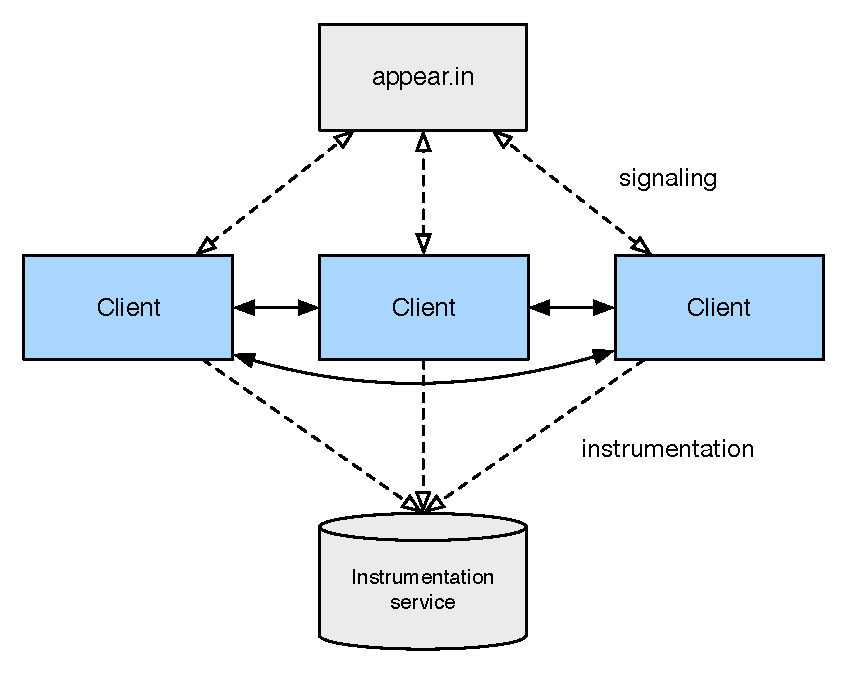
\includegraphics[width=0.9\textwidth]{Figures/appearin-arch}
    \caption{The appear.in architecture, illustrated for a conversation between 3 peers. \\ The black arrows indicate media data flow, and the dashed arrows indicate metadata flow: signaling data and instrumentation data, respectively.}
    \label{fig:appearin-arch}
\end{figure}

The instrumentation service has been included, simply to illustrate the fact that the data we have available is generated and sent directly from the clients.

By ``signaling'' in the context of appear.in, we mean everything not directly related to the media streams between the peers. This includes:

\begin{itemize}
  \item Managing which peers are in which room.
  \item Setting up new peer connections when a client joins a room.
  \item Tearing down peer connections when a client exits a room.
  \item Distributing various metadata that needs to be in sync across peers.
\end{itemize}

The user interface is also quite simple. It consists of a landing page (a screenshot of the current version can be seen in figure~\ref{fig:appearin-landing}), and a ``room page'' (see figure~\ref{fig:appearin-room}). For the sake of simplicity, let's go through them separately.

\subsubsection{The landing page}

\begin{figure}[h]
  \centering
    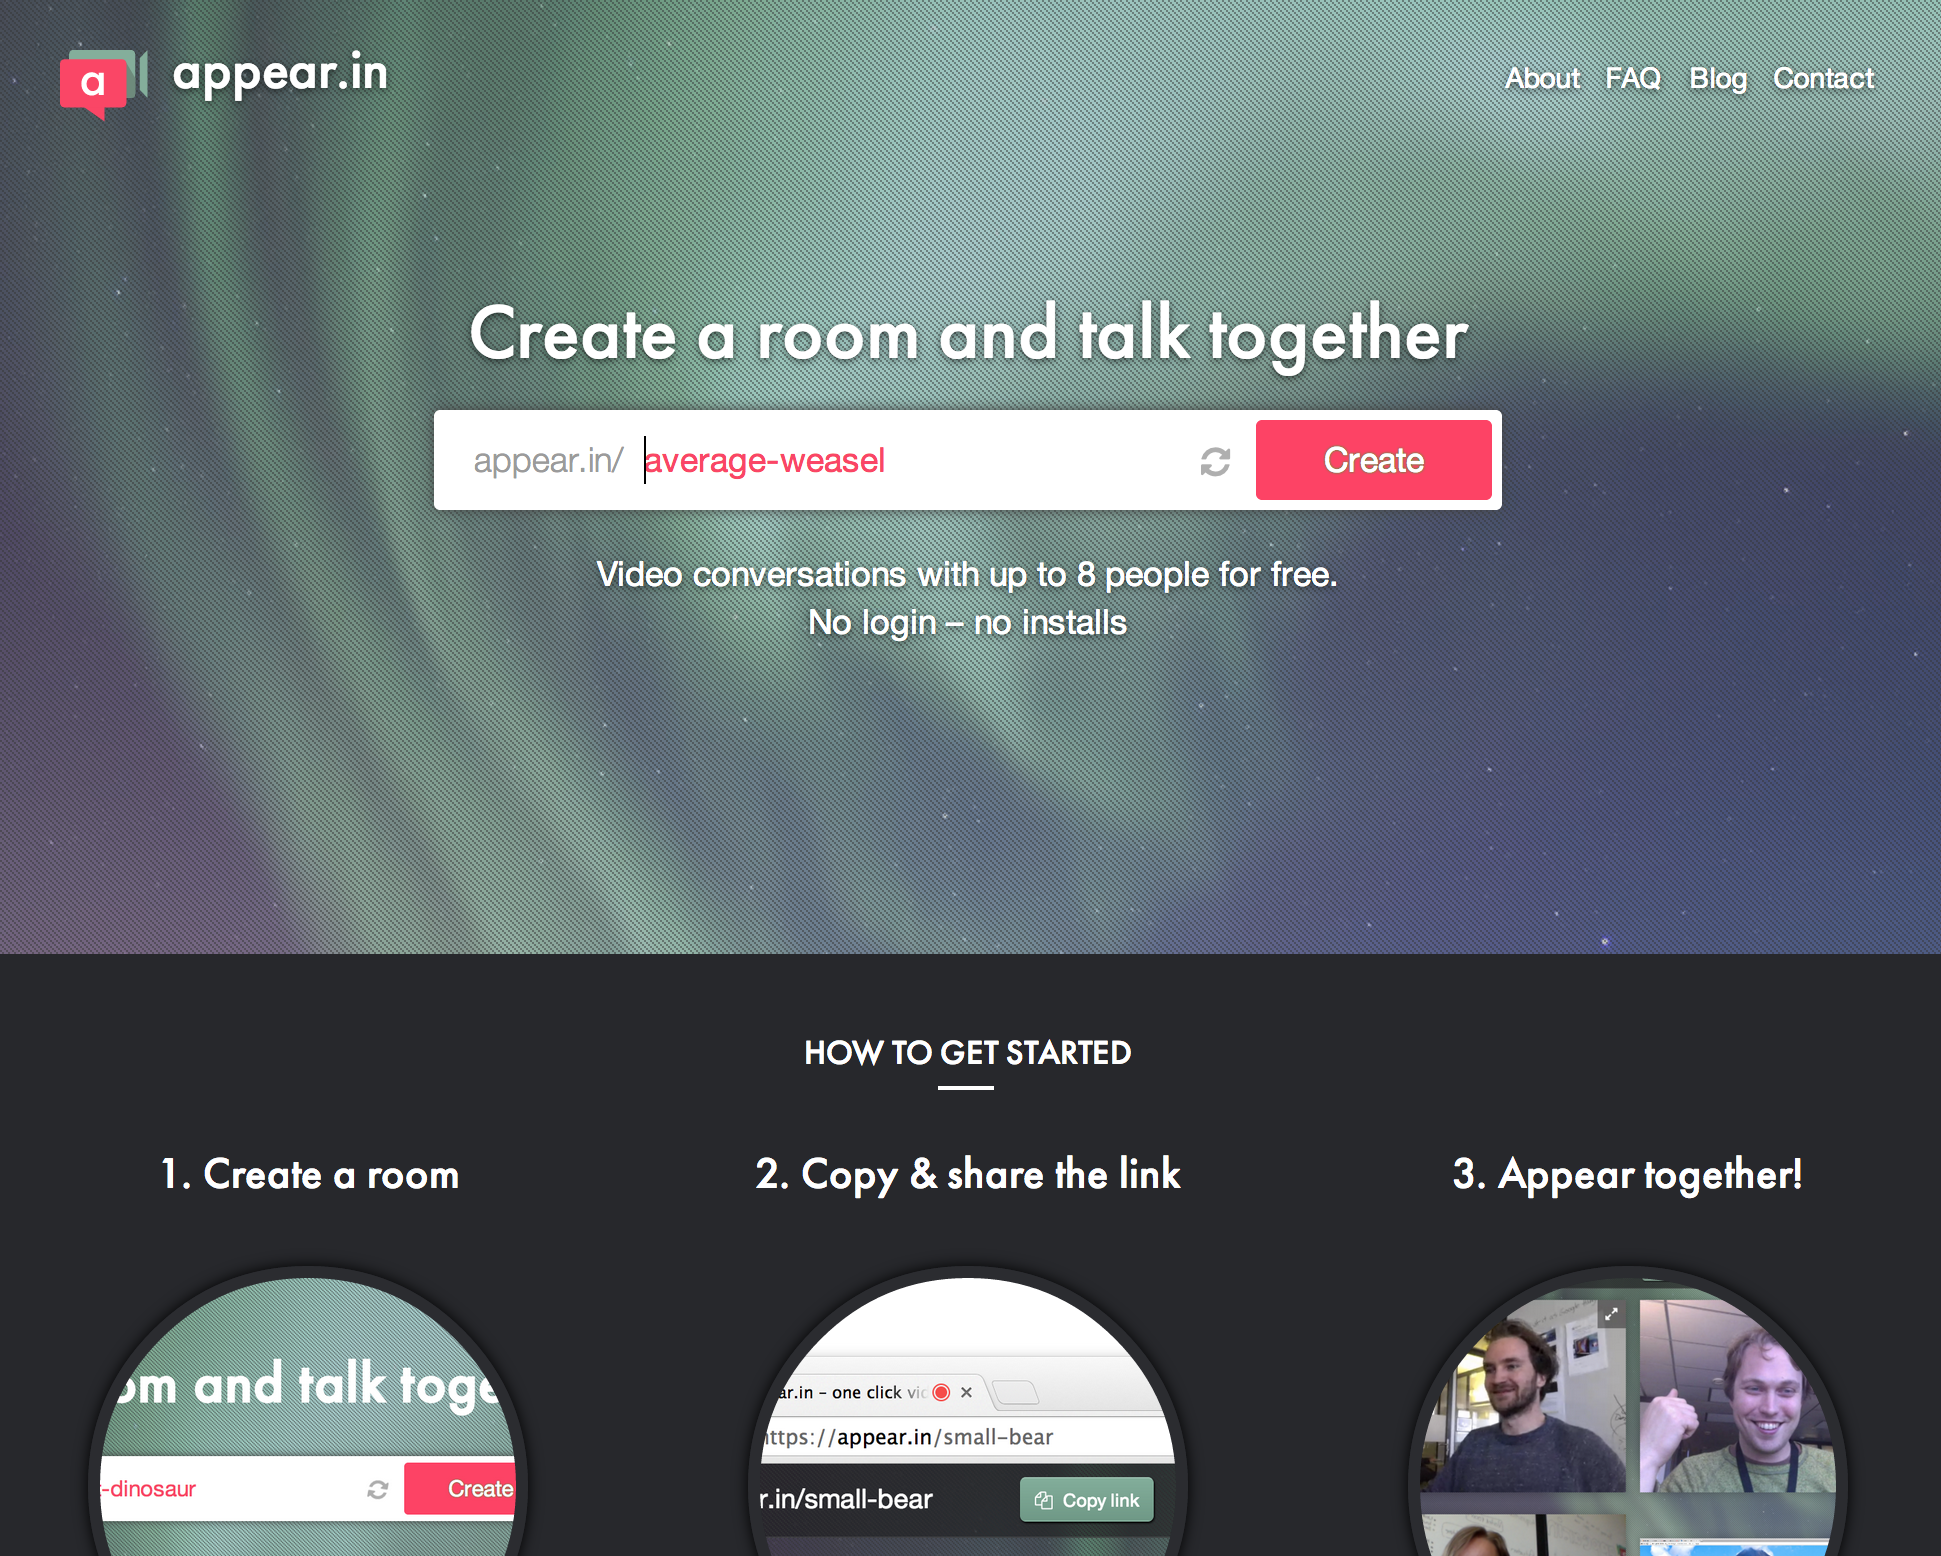
\includegraphics[width=\textwidth]{Figures/screenshots/appearin/frontpage-v2}
    \caption{The appear.in landing page (as of \today).}
    \label{fig:appearin-landing}
\end{figure}

The landing page's objective, as for most landing pages, is two-fold: to \emph{evoke interest}, and to \emph{activate the user}. Although we cannot directly measure them, we can indirectly measure the degree of interest and the activation rate in two ways:

\begin{enumerate}
  \item The ratio of users going from the landing page to a room (interest).
  \item The ratio of users going from the landing page to a room to a conversation (activation).
\end{enumerate}

The concept of evoking interest and of activating the user are universal terms that should generalize well to many other web applications.

\subsubsection{The room page}

\begin{figure}[t]
  \centering
    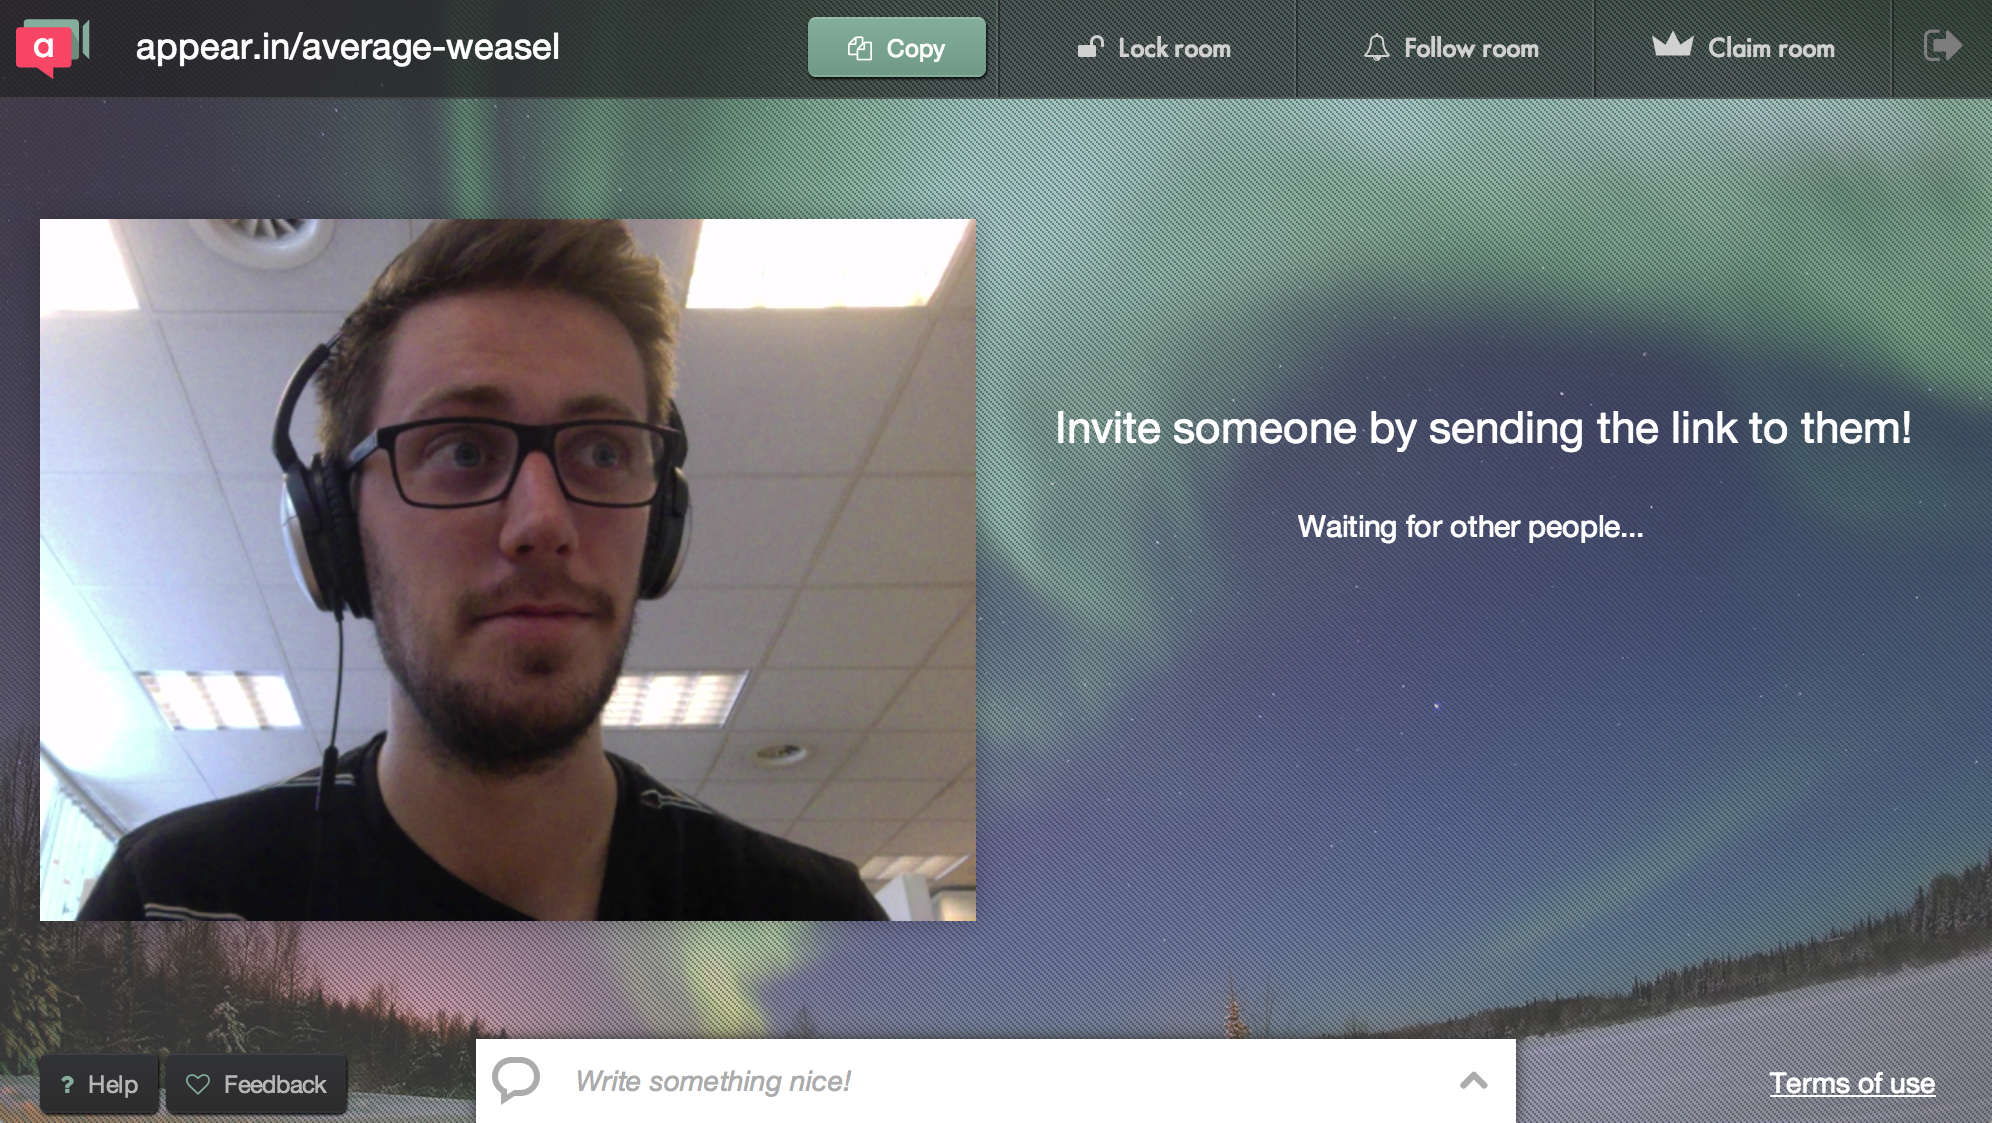
\includegraphics[width=\textwidth]{Figures/screenshots/appearin/in-room}
    \caption{The author in an appear.in room (as of \today).}
    \label{fig:appearin-room}
\end{figure}

The room page, the actual product user interface, is composed of several parts. Each participant resides in his or her own video control, and various room controls are placed along the top and bottom parts of the page.

As the quality of the video conferencing part of the application is largely governed by the browser and other low-level technicalities, we will mostly focus our efforts on the functionality augmenting the content: effectively, the rest of the UI.

\emph{Please note that all features discussed in this section are continuously subject to heavy revision, and should not in any way be viewed as a permanent or final set of features.}

The leftmost part of the top bar consists of a URL copying control, as shown in figure~\ref{fig:ui:copy_control}. Many users utilize this area when copying the page URL to invite their peers to the room. However, seeing as the same effect is easily achieved by copying the address field of the browser -- which we cannot track -- use of this control does not give a complete picture of users' sharing behavior.

To the top right is a row of buttons, as shown in figure~\ref{fig:ui:top_buttons}. Respectively, they allow the user to ``lock'', ``follow'', ``claim'', and leave the room. Of these, only the first three are of particular interest, as the ``leave room'' button essentially does nothing but close the window, severing the connection.

All these buttons alter the state of the room. Let's briefly walk through them.

\begin{description}
  \item[Lock] \hfill \\
    When locking a room, one prevents other people who stumble upon the room's URL from entering.\footnote{They are, however, able to knock their way in, much in the same fashion as one would enter a locked room in the physical world.}
  \item[Follow] \hfill \\
    Users following a room are notified when other people enter it. A room's followers may also follow the room chat without being present in the room, by using a browser extension.
  \item[Claim] \hfill \\
    Users can claim a previously unclaimed room, and essentially take ownership of it. This enables them to customize the room in a number of ways.
\end{description}

The last piece of the feature puzzle is the chat control, depicted in figure~\ref{fig:ui:chat}. When users post a message, it becomes visible to other members. Chat messages are written to a centralized store, and persist as long as there are people in the room.

\begin{figure}[t]
  \centering
  \begin{subfigure}[t]{0.8\textwidth}
    
\includegraphics[width=\textwidth]{Figures/screenshots/appearin/feature-copy}
    \caption{The room URL copying control.}
    \label{fig:ui:copy_control}
  \end{subfigure}

  \vspace{.5cm}

  \begin{subfigure}[t]{0.95\textwidth}
    
\includegraphics[width=\textwidth]{Figures/screenshots/appearin/feature-buttons-top}
    \caption{The top button row. Each button serves its own purpose and fires its own event.}
    \label{fig:ui:top_buttons}
  \end{subfigure}

  \vspace{.5cm}

  \begin{subfigure}[t]{0.95\textwidth}
    
\includegraphics[width=\textwidth]{Figures/screenshots/appearin/feature-chat}
    \caption{The chat control.}
    \label{fig:ui:chat}
  \end{subfigure}

  \caption{The most important UI parts.}
  \label{fig:important_ui_parts}
\end{figure}

\subsection{Generality of the application case}
\label{survey:sub:generality}

To improve our ability to generalize the functionality described in the previous section, we will focus on the application features augmenting the main video conferencing functionality. These functions essentially either \emph{manipulate the room resource} or aid in \emph{exporting information} about it. Thus, the analyzed feature set should apply equally well to other applications where these are central user tasks.

However, as touched upon in section~\ref{intro:sec:appearin}, the \emph{main} challenge of appear.in as an adaptation use-case is 1) the absence of demographics, and 2) the unreliability of user identity. The next sections look at how well these aspects generalize.

\subsubsection{The absence of demographics}

A key facet of all user adaptation and personalization is adapting to a user's interests, and so it is imperative to learn about the user. Montgomery and Srinivasan introduce a distinction between active and passive learning to aid in categorizing approaches to the issue~\cite{Montgomery2002}. Whereas active learning results from direct questions to the user, passive learning is the opposite: learning about the user without asking.

Active learning has several disadvantages in the general case:

\begin{enumerate}
  \item It requires too much effort on the customer's part.
  \item The user may indeed not know the answer to the questions, either lacking the proper knowledge or experience to evaluate the alternatives.
  \item The user may be unwilling to reveal correct answers.
  \item It is inefficient, as it typically ignores information consumers reveal about their preferences in their past interactions and purchases.
\end{enumerate}

The first point applies especially to the case of appear.in. An important part of the product is the simplicity of the application, ie. the small amount of friction. Thus, introducing questionnaires or similar approaches to collecting active feedback from users has not been viewed as a positive tradeoff up to this point.

So, we will be limited to passive learning. What does this leave us with in practice?

Montgomery identifies three major sources of information from which it is possible to learn passively: transaction data, clickstream data, and email.

appear.in, being a so-called single-page web application (SPA), has no clickstream in the traditional sense, a traditional clickstream being the series of pages navigated to. Transactional data, on the other hand, is usually related to e-commerce, and to some sense of ``items bought''. This is similarly irrelevant in this particular interpretation. However, we \emph{can} choose to view the series of interactions with the application as a clickstream of sorts -- an event stream -- and use it as a data source in much the same way.

\subsubsection{The unreliability of user identity}
\label{survey:unreliable_identity}

Being an anonymous service, appear.in has no explicit login. As explained in section~\ref{intro:sub:tracking_users}, appear.in uses cookies to track users over time, which introduces some challenges when it comes to building user models.

As we shall see, most users periodically clear their browser cookies (see~\ref{survey:sec:privacy_vs_personalization} for numbers), which causes an abrupt end of the perceived event stream from the browser user, never to be reassumed. The effect is illustrated in figure~\ref{fig:clear_cookie_impact} for a hypothetical case, in which user $A$ clears the browser cache twice, effectively cutting off the event stream each time. There is no obvious way in which to consolidate the three event streams of the three perceived users $A$, $B$, and $C$.

\begin{figure}[h]
  \centering
    \begin{subfigure}[t]{0.8\textwidth}
      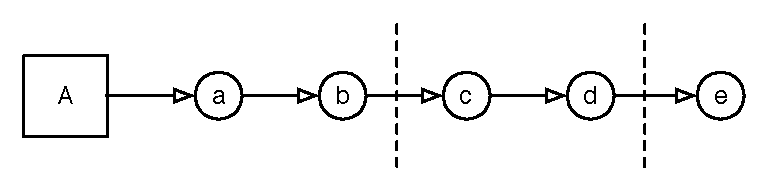
\includegraphics[width=\textwidth]{Figures/event-flow-cache-break-1}
      \caption{An event flow from $a \rightarrow e$, as seen from a user $A$. The dashed vertical lines indicate a point at which the user clears the browser cache.}
      \label{fig:cache_break1}
    \end{subfigure}
    \begin{subfigure}[t]{0.8\textwidth}
      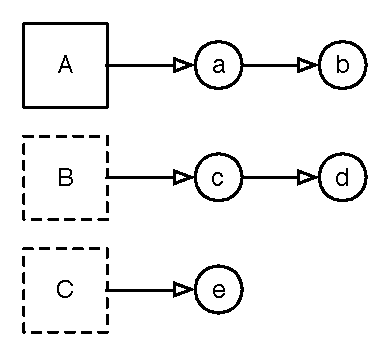
\includegraphics[width=0.5\textwidth]{Figures/event-flow-cache-break-2}
      \caption{The same event flow as perceived by the system.}
      \label{fig:cache_break2}
    \end{subfigure}

    \caption{The impact that clearing the browser cookies has on the chronological event stream for a single user $A$.}
    \label{fig:clear_cookie_impact}
\end{figure}

In practice, this leads to sparse usage data and quite a bit of noise in the event stream used as the basis for the user model generation. Furthermore, the shortening of event streams also introduces a bias to the clustering algorithms, as the user model vectors will be shorter than is actually the case. We will return to how this issue affects our approach in section~\ref{approach:sec:clustering}.

These are all issues that apply especially to appear.in, but that may also apply to many other anonymous systems.

\section{The field of user adaptation}
\label{survey:sec:user_adaptation}

This section will present an overview of the field of user adaptation. From the rather short history of the field, we move on to the conceptual frameworks and methodologies that modern adaptive systems base themselves on, before surveying the state of the art applications.

\subsection{A brief history of adaptive systems}
\label{survey:sec:adaptive_systems_history}

Vrieze discerns the history of adaptive systems into three eras~\cite{Vrieze}: early research, the pre-Internet era, and the Internet era. His historical dissertation is loosely based on Kobsa~\cite{Kobsa2001}. This summary will do the same, but the main focus of attention will be on what Vrieze calls \emph{the Internet era}, which is when user modeling and the Internet began to join forces.

\subsubsection{Early research}

The first work within user modeling research was conducted in the nineteen-eighties. Strongly influenced by the field of artificial intelligence, the groundwork for modern user modeling was laid.

The common denominator for the user modeling systems composed in this era was their tight integration with their respective production systems. The end of the era, however, saw systems such as GUMS~\cite{Finin1989}, the first standalone user modeling system. These early standalone systems are most widely known as User Modeling Shell Systems, a term coined by Kobsa in 1990~\cite{Kobsa1990}.

\subsubsection{Pre-Internet research}

The nineteen-nineties was a decade widely dominated by User Modeling Shell Systems, which carried on the tradition of GUMS from 1989. Mostly, stereotype-based approaches were used, which sought to deduce logical connections between user models and the application domain.

One system, however, Doppelgänger~\cite{Orwant1995}, stands out in this regard, being the only system to employ a probabilistic model, and not a logic-based approach~\cite{Kobsa2001,Pohl1997,Pohl1999}.

\emph{@TODO: Architecture underlining the ``pre-Internet'' name?}

\subsubsection{Internet-time research}

@TODO: What are recent developments and key enablers?

\subsection{Personalization on the web}
\label{survey:sub:web_personalization}

When the field of user adaptation meets the web, we have traditionally tended to dub it either ``web personalization'' or ``adaptive hypermedia''. The terms are defined as follows:

\begin{description}
    \item[Web personalization] \hfill \\
      Any action that adapts the information or services provided by a Web site to the needs of a particular user or a set of users, taking advantage of the knowledge gained from the users' navigational behavior and individual interests, in combination with the content and the structure of the Web site~\cite{Eirinaki2003}.
    \item[Adaptive hypermedia] \hfill \\
      A hypertext or hypermedia system, with a user model, able to adapt the hypermedia using the model~\cite{Brusilovsky1996}.
\end{description}

The first of these definitions assumes the website to be a hierarchy of content. However, large parts of the modern web have indeed shifted towards the application domain, as discussed in section~\ref{intro:sub:the_modern_web}. The traditional concept of a website being some kind of structured set of ``content pages'' is completely outdated. In this light, the definition of web personalization is a bit dated.

Adaptive hypermedia, on the other hand, is a wide and general enough term to cover our application case, and much research within its scope applies well to our application case.

We will be using the terms ``user adaptation'' and ``personalization'' without relating it to the domain in which it is visible to the user, as this is quite irrelevant where a clear separation of the application and adaptational component is in place. However, as the ``hypermedia'' term implies, we base our adaptations on interactions with the interface.

The evolution of these models through the 90s and into the modern internet era is elaborated on in the following sections.

\subsection{Implementation methodology}

As mentioned, there are many approaches to the task of user adaptation. Due to the constraints outlined in the previous chapters, we will be honing in on the approach termed ``web usage mining'', or sometimes ``clickstream analysis''.

Traditionally, this has entailed tracking the way users traverse a website hierarchy, looking for path patterns among them, and using this information to adapt the pages in various ways~\cite{Mobasher2000,Eirinaki2003,Montgomery2009}. While not entirely the same task, this is mostly analogous to the type of adaptation problem we are solving, and the systems proposed in this earlier work solves many of the same problems that this work will need to solve.

% The following belongs in history, if anywhere. Outdated figure.
%
% A general, high-level sketch of a typical adaptive system is outlined in figure~\ref{fig:general_adaptive_system}.
%
% \begin{figure}[h]
%   \centering
%     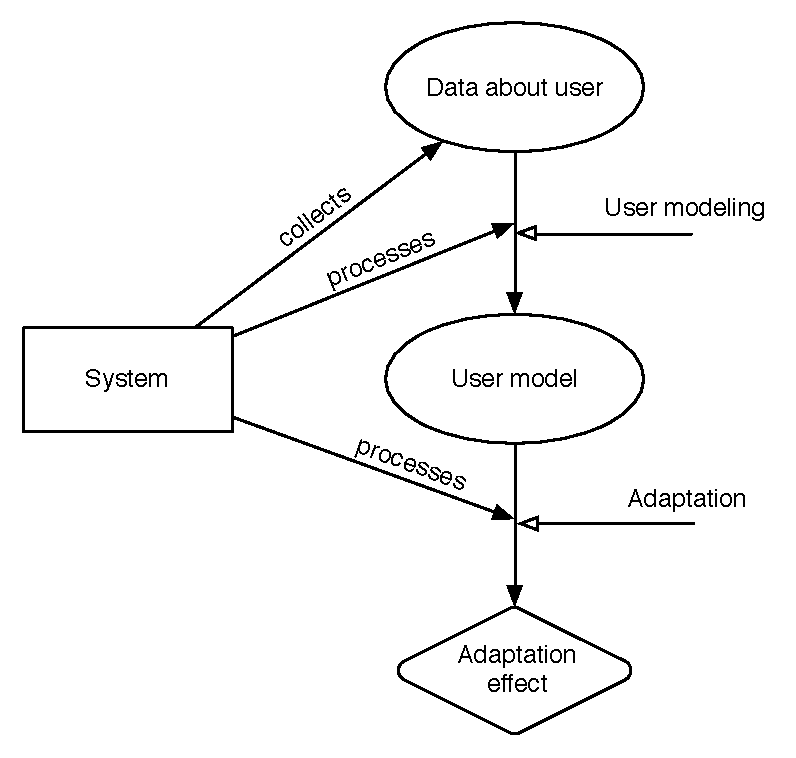
\includegraphics[width=0.8\textwidth]{Figures/adaptation-high-level}
%   \caption{Caption.}
%   \label{fig:general_adaptive_system}
% \end{figure}

\subsection{Privacy versus personalization}
\label{survey:sec:privacy_vs_personalization}

The marketing firm Jupiter defines personalization as ``predictive analysis of consumer data used to adapt targeted media, advertising and merchandising to consumer needs. According to Jupiter, personalization can be viewed as a cycle of recurring processes consisting of \emph{data collection}, \emph{profiling} and \emph{matching}''~\cite{Foster2000}. This section will discuss some ethical and political issues surrounding the first step of this cycle, namely \emph{data collection}.

Teltzrow and Kobsa~\cite{Teltzrow2004} state it plainly: ``Personalization systems need to acquire a certain amount of data about users' interests, behavior, demographics and actions before they can start adapting to them.'' As we shall see, many Internet users are highly sceptical of providing personal information to web sites, and a majority are concerned about web sites tracking their movements and behavior online. This doesn't fit adaptive systems' demand for data collection.

\subsubsection{Personal information}

First, consider the following survey results regarding personal infomation~\cite{Teltzrow2004}:

\begin{enumerate}
  \item Internet Users who are concerned about the security of personal information: 83\%~\cite{CyberDialogue2001}, 70\%~\cite{Behrens2001}, 84\%~\cite{Fox2000}
  \item People who have refused to give (personal) information to a web site: 82\%~\cite{Culnan2001}
  \item Internet users who would never provide personal information to a web site: 27\%~\cite{Fox2000}
  \item Internet users who supplied false or fictitious information to a web site when asked to register: 34\%~\cite{Culnan2001}, 24\%~\cite{Fox2000}
\end{enumerate}

Although the above numbers aren't directly relevant to the case of appear.in, where no personal information is collected or stored, it underlines a general scepticism towards providing information to web sites.

The fact that such a large portion of users are sceptical of providing personal data tells us that there is reason to believe there is room for anonymous niches within most application areas, serving as a drive towards more applications like appear.in.

\subsubsection{Tracking}

The same scepticism as above is again seen when users are surveyed on their attitudes towards being tracked online~\cite{Teltzrow2004}.

\begin{enumerate}
  \item People who are concerned about being tracked on the Internet: 60\%~\cite{CyberDialogue2001}, 54\%~\cite{Fox2000}, 63\%~\cite{Harris2000}
  \item Internet users who generally accept cookies: 62\%~\cite{PersonalizationConsortium2000}
  \item Internet users who set their computers to reject cookies: 25\%~\cite{Culnan2001}, 3\%~\cite{CyberDialogue2001}, 31\% in warning modus~\cite{CyberDialogue2001}, 10\%\cite{Fox2000}
  \item Internet users who delete cookies periodically: 52\%~\cite{PersonalizationConsortium2000}
\end{enumerate}

As discussed in section~\ref{survey:unreliable_identity}, any time a user clears the browser cookies, we effectively break the user's event stream, and is from that moment onwards -- for all we know -- a brand new user.

This makes it hard to know if these numbers are similar to those among the users of appear.in, as they have not yet been surveyed on this subject. Furthermore, our only data source touching the user base is based on the tracking cookies in question -- hence we are unable to examine to what extent the above survey applies to our case.

\subsubsection{The road ahead}

Although these numbers are a bit dated, there is little reason to believe that the tracking situation is going to get any easier in the years to come~\cite{RuizMartinez2012,Nikiforakis2013,Sorensen2013,Eijk2011}.

As we have seen, there already exists broad scepticism towards the use of cookies to track users, even on first-party sites. Much of the problem seems to stem from sites allowing third-party cookies, to better serve advertisements to its users -- who most often are oblivious to the tracking taking place at all.

These third-party cookies, however, allow these third-parties to track users' activity and behavior across multiple sites, often without their explicit consent. This has recently been deemed as bordering to surveillance, and in recent years extensive legislative restrictions have been introduced to decrease the prevalence of particularly third-party cookies.

This all presents a challenge for services like appear.in, who use third-party cookies not to advertise, but to enhance the service for the user. There is reason to believe this situation will not become easier to deal with in the years to come, but hopefully, there will come about better ways of dealing with the issue.

\section{Clustering techniques}
\label{survey:sec:clustering_techniques}

There are many approaches to the task of clustering user models.

@TODO: Some text on hierarchical, flat, density, probabilistic, k-median etc, before presenting k-means as our choice due to: good match with both input and desired output, scales well (parallel optimization), by far most popular in commercial applications~\cite{Berkhin2006}.

\subsection{Clustering evaluation}
\label{survey:sub:clustering_evaluation}

In general, any clustering method should search for clusters whose members are close to each other and well separated. Berry and Linoff~\cite{Berry1996} formulate it in terms of \emph{compactness} and \emph{separation}.

\begin{description}
  \item[Compactness] \hfill \\
    The members of each cluster should be as close to each other as possible.
  \item[Separation] \hfill \\
    The clusters themselves should be widely spaced.
\end{description}

For an algorithm such as $k$-means, which takes the $k$ as an input, the central question when it comes to cluster validity is for which value of $k$ the cluster compactness and separation are optimal.

The most efficient way of measuring cluster quality between several executions of a clustering method, where only its parameters -- like $k$ -- differ, is to utilize a so-called \emph{relative criteria}~\cite{Halkidi2001}.

One of the most widely used measures of clusters' relative criteria is the Davies-Bouldin index, which is the one used to differentiate between clusters in this project. It is defined as:

\begin{equation}
  \text{DB}_k = \frac{1}{k} \sum_{i=1}^k \max_{i \neq j} \left( \frac{s_i + s_j}{d(c_i, c_j)} \right)
\end{equation}

where $k$ is the number of clusters, $c_x$ is the centroid of cluster $x$, $s_x$ is the average distance of all elements in cluster $x$ to centroid $c_x$, and $d(c_i,c_j)$ is the distance between centroids $c_i$ and $c_j$.

In plainer words, the Davies-Bouldin index formulates a measure of the quality of cluster separation and compactness, while considering the number of clusters in a responsible manner. Thus, it is well suited to distinguish between runs of eg. the $k$-means algorithm, where the value of $k$ differs from run to run.

\section{A/B testing}
\label{survey:sec:ab_testing}

Controlled experiments embody the best scientific design for establishing a causal relationship between changes and their influence on user-observable behavior~\cite{Kohavi2007,Kohavi2008}.

The simplest form of controlled experiment is often referred to as the A/B test. In A/B tests users are randomly exposed to one of two variants: control (A), or treatment (B). Based on data collected, an Overall Evaluation Criterion (OEC) is derived for each variant. Figure~\ref{fig:ab_flow} illustrates the A/B testing process.

\begin{figure}[h]
  \centering
    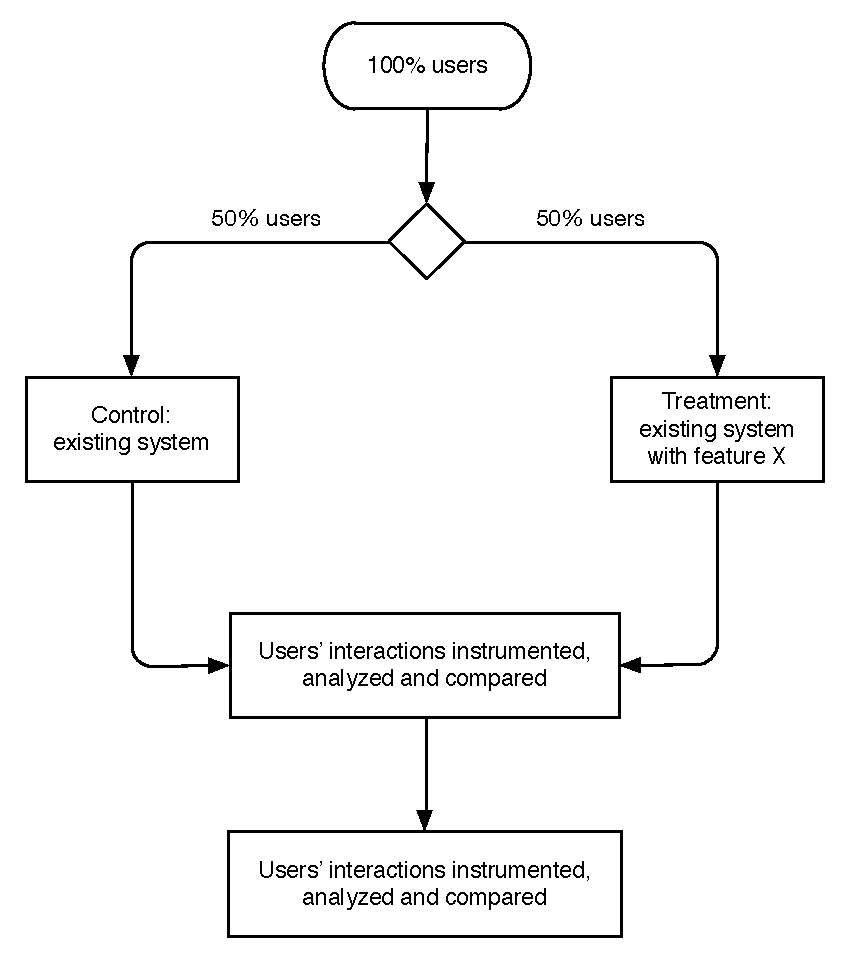
\includegraphics[width=0.7\textwidth]{Figures/ab-test-flow}
    \caption{The flow of an A/B test.}
    \label{fig:ab_flow}
\end{figure}

One word in the previous paragraph, ``randomly'', warrants some discussion. To be able to establish a causal relationship between the selected variant and the evaluation, the variant selection must indeed be completely random, and not based on what Kohavi et al. term ``any old which way''~\cite{Kohavi2007}.

This point \emph{must} be kept in mind when designing adaptive systems based on controlled experiments, as in our case.

\section{State of the art}
\label{survey:sub:state_of_the_art}

\emph{@TODO: Compile a set from the above sections.}

\chapter{Approach}

\label{Chapter3}

\lhead{Chapter 3. \emph{Approach}}

\section{System overview} % (fold)
\label{sec:system_overview}

The proposed system is constructed around the data flowing through it.

The system takes the data stepwise through an ingestion pipeline, importing, filtering and cleaning it, before churning it into user models. This particular part of the system is elaborated on further in section~\ref{sec:data_ingestion_and_preprocessing}.

Once user models are in place, the system generates user segments. These are stored in a database for future use. There are several viable approaches to the segmentation task. These are discussed in more detail in section~\ref{sec:clustering}.

As it turns out, when designing completely autonomous adaptative systems, we need more data than user segments to effectively drive the adaptive component. When considering whether to enable a feature or an interface switch, we need to know whether doing so will be advantageous to the user segment in question. This is discussed in section~\ref{sec:adaptation_component}.

% section system_overview (end)

\section{Data ingestion and preprocessing} % (fold)
\label{sec:data_ingestion_and_preprocessing}

Before the interesting parts of the system can start doing their work, the data needs to be transformed from \emph{a series of chronological raw events} to \emph{a set of user models}.

The amount of data can be arbitrarily sizable, and will grow linearly with user activity. The system architecture has been designed to be able to cope with this; its functional and data-driven nature should be easily adaptable to hugely scalable programming paradigms like MapReduce.

\begin{figure}[h]
  \centering
    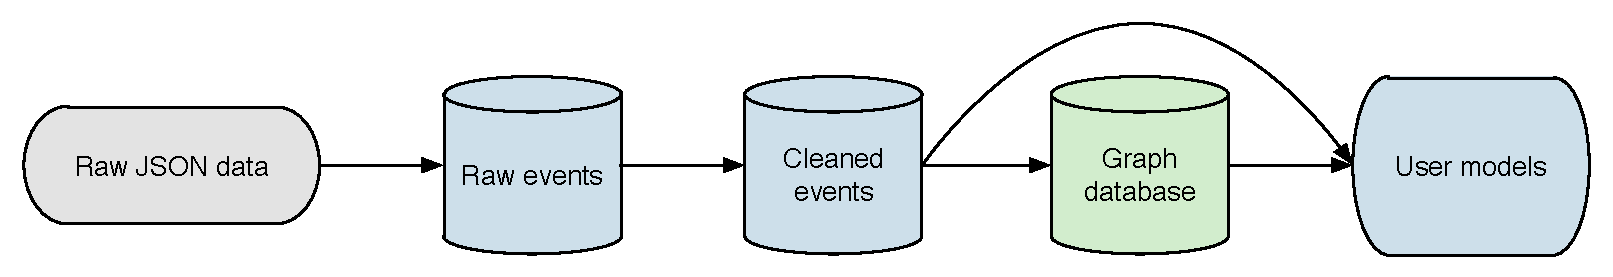
\includegraphics[width=\textwidth]{Figures/ingestion-pipeline}
  \caption{The ingestion pipeline broken into 4 steps. The color of each node indicates means of storage: \emph{Blue} indicates a RDBMS, \emph{green} indicates a graph database, whereas \emph{gray} is used to indicate flat file storage.}
  \label{fig:ingestion-pipeline}
\end{figure}

\subsection{Generating the raw data}
\label{sub:generating_data}

The system input is a chronological series of raw events sent from the production system.

These are instrumented via an external analysis service called KISSmetrics\footnote{\url{https://www.kissmetrics.com/}}. It is a user analysis system designed around tracking individual users' behavior. It works by calling their REST API with the following data:

\begin{enumerate}
  \item person identifier
  \item event name
  \item user properties
\end{enumerate}

The consistency of the personal identifier has already been discussed extensively in the introductory chapters, especially section~\ref{sub:anonymity_privacy}, but a short technical introduction to the actual production system is in order.

\subsection{Event instrumentation in KISSmetrics}
\label{sub:event_instrumentation}

To enable effective utilization of the KISSmetrics instrumentation functionality, they supply a client library for the purpose. This client library handles a few central things for us:

\begin{enumerate}
  \item Person identity storage and loading over subsequent page loads.
  \item The low-level instrumentation of events.
  \item Simple A/B testing facilities.
\end{enumerate}

When the KISSmetrics client library is loaded, the person identity is automatically either retrieved from the browser cookies, or generated.

The identity of a person is a unique randomly generated string, which serves no other purpose than to track the identity of the browser over time. No personal data is stored, nor is it available to us.

Whenever something ``interesting'' happens, an event is sent to the KISSmetrics instrumentation service. An ``interesting'' event is anything that tells us about how the users use the service, both in terms of general activity and in terms of feature adoption. Every event is tagged with the person identity, as well as an event name and a timestamp.

The KISSmetrics service provides several analytical tools to dig into this data, thereamongst funnel reports and cohort reports -- as depicted in figure~\ref{fig:funnel-report} and figure~\ref{fig:cohort-report}.

\begin{figure}[h]
  \centering
    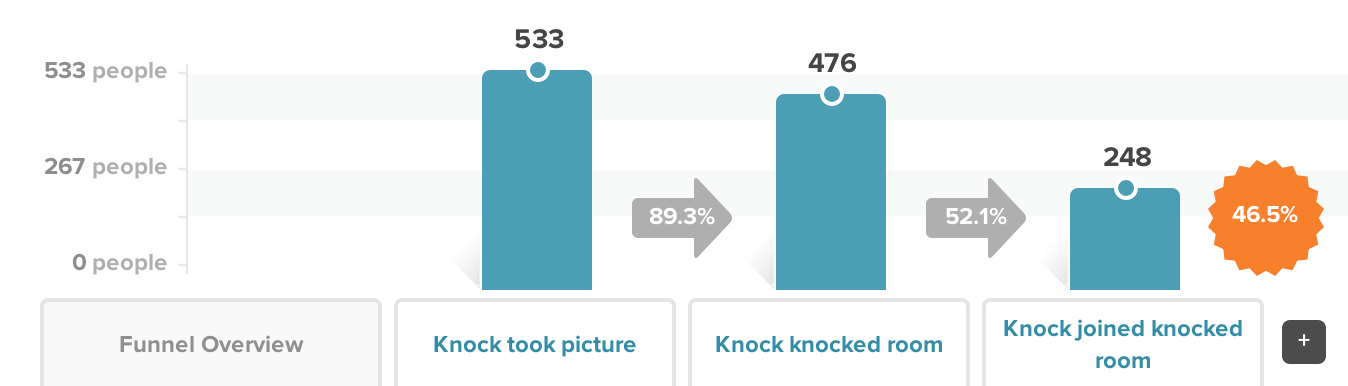
\includegraphics[width=\textwidth]{Figures/screenshots/km/funnel-example}
    \caption{Example of a simple funnel report.}
    \label{fig:funnel-report}
\end{figure}

\begin{figure}[h]
  \centering
    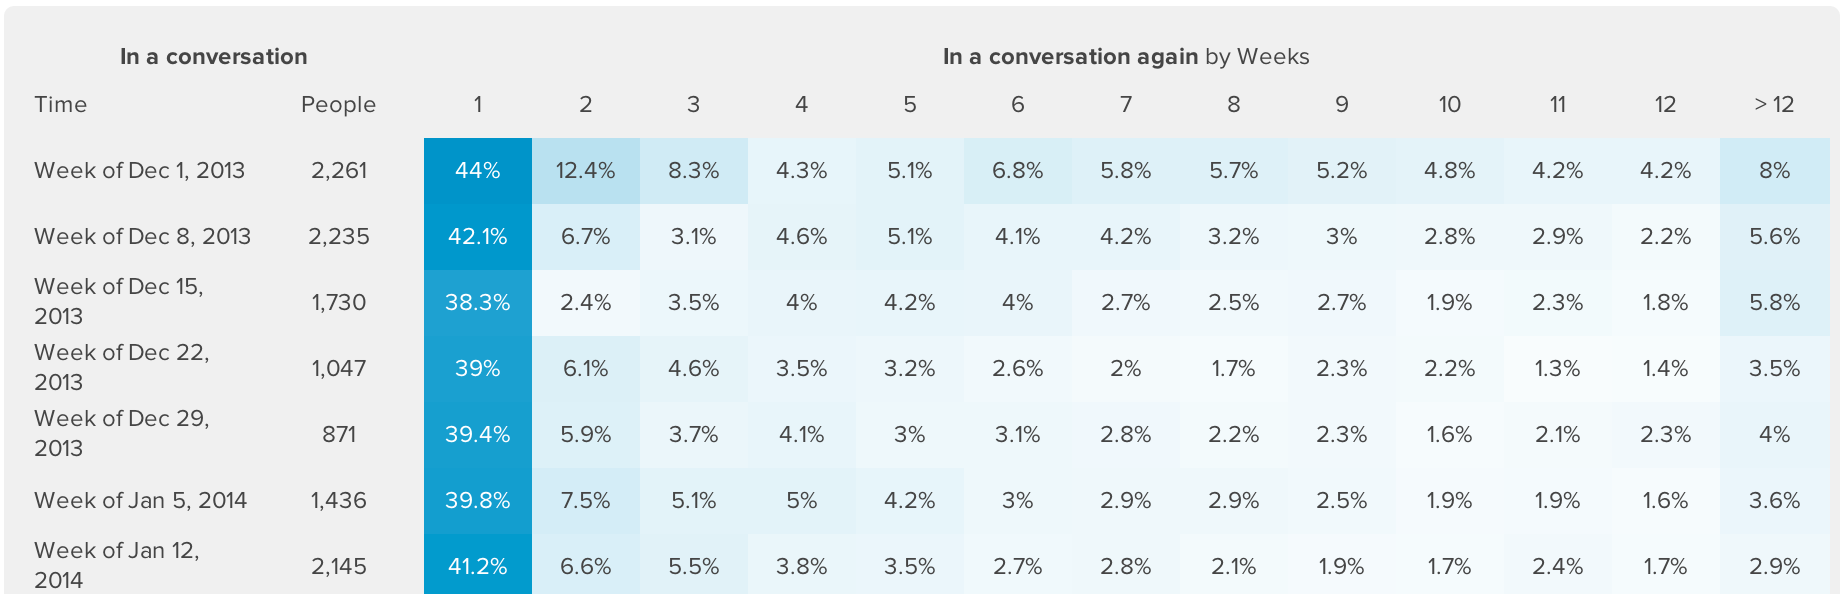
\includegraphics[width=\textwidth]{Figures/screenshots/km/cohort-example}
    \caption{Example of a cohort report.}
    \label{fig:cohort-report}
\end{figure}

\subsection{Cleaning the data}
\label{sub:cleaning_data}

KISSmetrics has the ability to export raw event data to data files. This can be used to power completely customized analyses, as will be needed for our particular task.

After the raw data has been aquired, it will need to be cleaned. This is a simple process of churning through each line of each unprocessed data file, parsing and splitting its contents into appropriate data fields, and inserting it into a database.

To facilitate the compilation of network-related user model features, conversation data was loaded into a graph database to enable querying of network structures. In the RDBMS handling the other data, this presented itself as a computationally unfeasable task.

% section data_ingestion_and_preprocessing (end)

\section{User modeling} % (fold)
\label{sec:user_modeling}

To find clusters of users, we first and foremost need to quantify them. More specifically, we want to represent each user as a feature vector in an $n$-dimensional space.

\subsection{Feature selection}
\label{sub:feature_selection}

Given the types of events being collected, we landed on compiling the following features:

\begin{enumerate}
  \item First degree conversation partners
  \item Second degree conversation partners
  \item Inviter
  \item Invitee
  \item Conversations
  \item Rooms used
  \item Rooms claimed
  \item Roomnames generated
  \item Chat message sent
\end{enumerate}

To generate user models, the stream of event data needs to be mapped to its associated users for aggregation. This is a classic MapReduce task~\cite{Dean2008} easily solved using simple functional techniques, and did not present itself as a particularly interesting problem, albeit a computationally heavy one.

To summarize, the transformation in this step started with data in the form of \eqref{pre_user_model}.

\begin{equation}
  \langle \text{event}, \text{timestamp}, \text{person}, \text{metadata} \rangle
  \label{pre_user_model}
\end{equation}

And ended with data in the form of~\eqref{post_user_model}.

\begin{equation}
  \langle \text{person}, \text{feature}, \text{value} \rangle
  \label{post_user_model}
\end{equation}

\section{Clustering the users}
\label{sec:clustering}

We assume the following hypothesis holds, as a basis for the clustering approach to the user adaptation problem:

\begin{hypothesis}
The more similarly two people use a service, the more likely they are to respond similarly to it changing.
\end{hypothesis}

Thus, we want to segment the users in the following way: users in each segment should be as similar as possible, and as dissimilar those in other segments as possible. This scheme fits well with the two criterias for selecting an optimal clustering scheme, as described by Berry and Linoff~\cite{Berry1997}.

\subsection{Choice of algorithms}
\label{sub:clustering_algorithms}

Three algorithms were implemented and experimented with: DBSCAN, mean-shift, and k-means. Of these, the k-means clearly proved itself as the most effective one, and as it also managed to produce adequate and meaningful results, it was chosen as the principal algorithm.

\subsubsection{The k-means clustering algorithm}
\label{subs:kmeans}

The k-means clustering algorithm is arguably one of the most intuitive clustering algorithms.

It takes as input a preset number of clusters, $k$, a similarity measure function, and a set of data vectors. Initially, it randomly chooses $k$ data vectors as centroids as a starting point for the process, before repeatedly performing a two-pass operation adjusting the centroids until convergence.

Figure~\ref{fig:k-means} shows a simple python-esque implementation of the algorithm.

\begin{figure}[h]
  \begin{minted}[gobble=4]{python}
    def kmeans(K, distance_fn, vectors):
        N = len(vectors)
        cluster_members = {}
        memberships = {}

        # Initially set centroids to random data vectors
        centroids = [vectors[randint(N)] for _ in xrange(K)]

        while True:

            # Assign each data vector to the closest cluster centroid
            for vector in vectors:
                k = argmin(K, lambda k: distance_fn(centroid[k], vector))
                if not memberships[vector] == k:
                    cluster_members[memberships[vector]].remove(vector)
                    cluster_members[k].append(vector)
                    memberships[vector] = k

            # Set each centroid to the mean of its members
            previous_centroids = centroids
            for k in xrange(K):
                centroids[k] = mean_vector(cluster_members[k])

            # Stop computing if we've achieved convergence
            change = 0.0
            for k in xrange(K):
                change += distance_fn(previous_centroids[k], centroids[k])
            if change < CONVERGENCE_THRESHOLD:
                break
  \end{minted}

  \caption{The k-means algorithm}
  \label{fig:k-means}
\end{figure}

\subsection{Evaluating cluster quality}
\label{sub:evaluating_clusters}

@TODO: Davies-Bouldin index etc.

\subsection{Normalizing axes}
\label{sub:normalizing_axes}

\subsection{Storing clustering results}
\label{sub:storing_results}

\section{Identifying adaptable product features}
\label{sec:identifying_adaptability}

Ideally at this point, we have identified several significant clusters of users. Now we want to adapt the product to better suit each user, based on the cluster he or she belongs to.

Given a set of candidate product alterations $A$, we want to give each user the combination of these that maximizes some performance measure $P$. However, we arguably have no predictive bias to start us off on solving this.

The approach taken in this implementation is a simple one, which relies on conducting a single A/B test up front for each candidate product alteration. The important part during this phase is to log each selected alteration variant along with the same person identifier used for other event instrumentation, as discussed in section~\ref{sub:generating_data}.

This approach enables us to see up-front whether there are any significant variances in feature adoption between the clusters. If there are, we can adapt the service by selecting the more successful variation of the feature for all users in the relevant clusters. If not, we have a feature that affects all users equally -- at least with regard to cluster granularity.

\subsection{Evaluation metrics} % (fold)
\label{sub:evaluation_metrics}

When considering which variation of a product feature to prefer, we need to be able to measure their relative success rates.

As for any user-facing product, the main objective is achieving user happiness. However, user happiness is hard to objectively define. For a service like appear.in, though, activity level should serve as a pretty clear indicator of user happiness -- unhappy users have more than enough alternative applications that cater to their needs.

Simply put, we basically assume that the following hypothesis holds:

\begin{hypothesis}
  Happy users use the service more than unhappy users.
\end{hypothesis}

Furthermore, we seldom need a measure of \emph{user happiness} to determine the relative success of variations of a product feature. Some parts of the product have clearly defined goals themselves.

The perhaps most obvious example of this is the landing page, whose main objective is to get people to try out the product. We can define the performance of the landing page in terms of the percentage of users that continue on to try out the product.

\section{Adaptation component} % (fold)
\label{sec:adaptation_component}


\subsection{Applying the personalized feature set} % (fold)
\label{sub:applying_the_personalized_feature_set}

Description of the FlagService model.

% section applying_the_personalized_feature_set (end)

\subsection{Visualizing effects} % (fold)
\label{sub:visualizing_effects}

% section visualizing_effects (end)

% section adaptation_component (end)

\subsection{Differentiating product features} % (fold)
\label{sec:differentiating_product_features}

% section differentiating_product_features (end)

\section{Evolving the user models} % (fold)
\label{sec:evolving_the_user_models}

\subsection{Multi-arm bandits}

\subsection{Tracking individual treatment}

% section evolving_the_user_models (end)

\section{Visualization requirements (?)} % (fold)
\label{sec:visualization_requirements}

% section visualization_requirements (end)

\chapter{Evaluation}

\label{Chapter4}

\lhead{Chapter 4. \emph{Evaluation}}

This chapter will evaluate the approach presented in chapter~\ref{Chapter3}, by implementing a prototype of the described system.

The chapter starts with introducing the main goal and the experimental setup in sections~\ref{eval:sec:prerequisites} and~\ref{eval:sec:experimental_setup},
before evaluating the actual results in sections~\ref{eval:sec:ab_testing_features},~\ref{eval:sec:clustering}, and~\ref{eval:sec:adapting_the_application}.
We round up the section with a summary and discussion, in sections~\ref{eval:sec:summary} and~\ref{eval:sec:discussion}.

\section{Prerequisites} % (fold)
\label{eval:sec:prerequisites}

For any of this user adaptation to have any actual use, we will need to find out whether there is actually significant variation in feature adoption between clusters; it matters little whether users exhibit differing behavior with regard to existing functionality, if this behavior yields no basis for predicting feature adoption in the future. We need an inductive bias.

An easy way of discovering whether this inductive bias is present in the user base is to simply log whether there is significant variance across the user groups in their users' adoption of new features. Thus, this question of whether the predictive bias actually exists will be included as a central part of the actual experiment itself, and be thoroughly discussed through the next sections.

% section prerequisites (end)

\section{Experimental setup} % (fold)
\label{eval:sec:experimental_setup}

\begin{figure}[h]
  \centering
    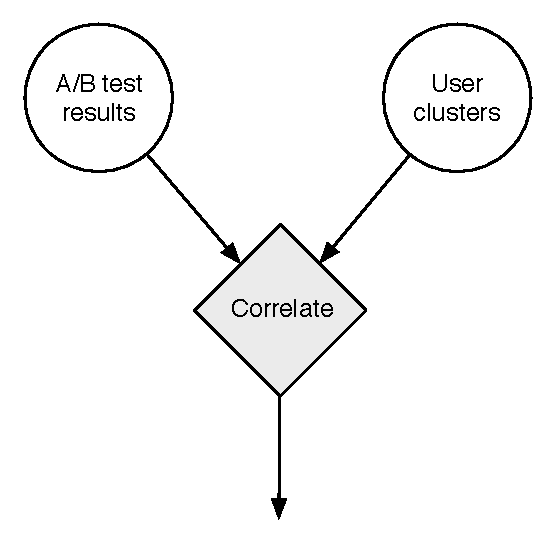
\includegraphics[width=0.5\textwidth]{Figures/experimental-setup}
    \caption{The experiment setup. The output of the correlation component (in gray) will determine the outcome of the experiment.}
    \label{fig:experimental-setup}
\end{figure}

The main experiment will determine whether an alteration of the service performs differently among ``different kinds of users''. A/B test results and user clusters will serve as input data to test the hypothesis.

@TODO: Formulate exact hypothesis.

The data from the A/B test results describe each person's designated variant, and the resulting performance. See table~\ref{tab:person_variants} for some example data.

\begin{table}[h]
  \centering
  \begin{tabular}{|llll|}
    \hline
    Person & Variant & Entered room & Entered conversation \\ \hline
    p1     & A       & no           & no  \\
    p2     & A       & yes          & yes \\
    p3     & B       & yes          & no  \\
    p4     & A       & no           & no  \\
    p5     & B       & yes          & yes \\ \hline
  \end{tabular}
  \caption{Each person has one assigned variant, and some performance measures.}
  \label{tab:person_variants}
\end{table}

The user cluster data contain the same persons as the test results in table~\ref{tab:person_variants} and the clusters they have been assigned to, as illustrated in table~\ref{tab:person_clusters}.

\begin{table}[h]
  \centering
  \begin{tabular}{|ll|}
    \hline
    Person & Cluster \\ \hline
    p1     & 1 \\
    p2     & 2 \\
    p3     & 1 \\
    p4     & 1 \\
    p5     & 2 \\ \hline
  \end{tabular}
  \caption{Persons have been assigned to to clusters.}
  \label{tab:person_clusters}
\end{table}

These data sources are aggregated with regard to variant and cluster, and the relative success rates compared.

--

\emph{Condensed version.}

The main experiment determines whether an alteration of the service affects different kinds of users differently.
More specifically, do users in clusters $C_1, \ldots, C_n$ employ function $f$ in significantly differing ways? We find out without touching a large percentage of the users, and can use the results to individually enable features for users that

We break the process into three steps, each elaborated on in~\ref{approach:sec:feature_experiments}, \ref{approach:sec:clustering}, and \ref{approach:sec:adaptation_component}:

\begin{enumerate}
  \item A/B test feature $f$ on a percentage of all users.
  \item Separate users into clusters $C_1, \ldots, C_n$.
  \item Analyze results: did the test results vary significantly between clusters?
\end{enumerate}

If the final answer is ``yes'', we can store our results and use them as a basis for adaptating the interface for each user.

\section{A/B testing features} % (fold)
\label{eval:sec:ab_testing_features}

Due to various reasons, there was only time to perform one controlled content experiment. However, it will illustrate the approach adequately.

\subsection{New appear.in landing page}
\label{eval:sub:new_landing_page}

The experiment stood between the old landing page, the control treatment, and a new design. We shall from here on refer to them as variation $A$ and $B$, respectively. The two competing variations are depicted in figure~\ref{fig:variations}.

\begin{figure}[h]
  \centering
    \begin{subfigure}[t]{0.8\textwidth}
      \centering
      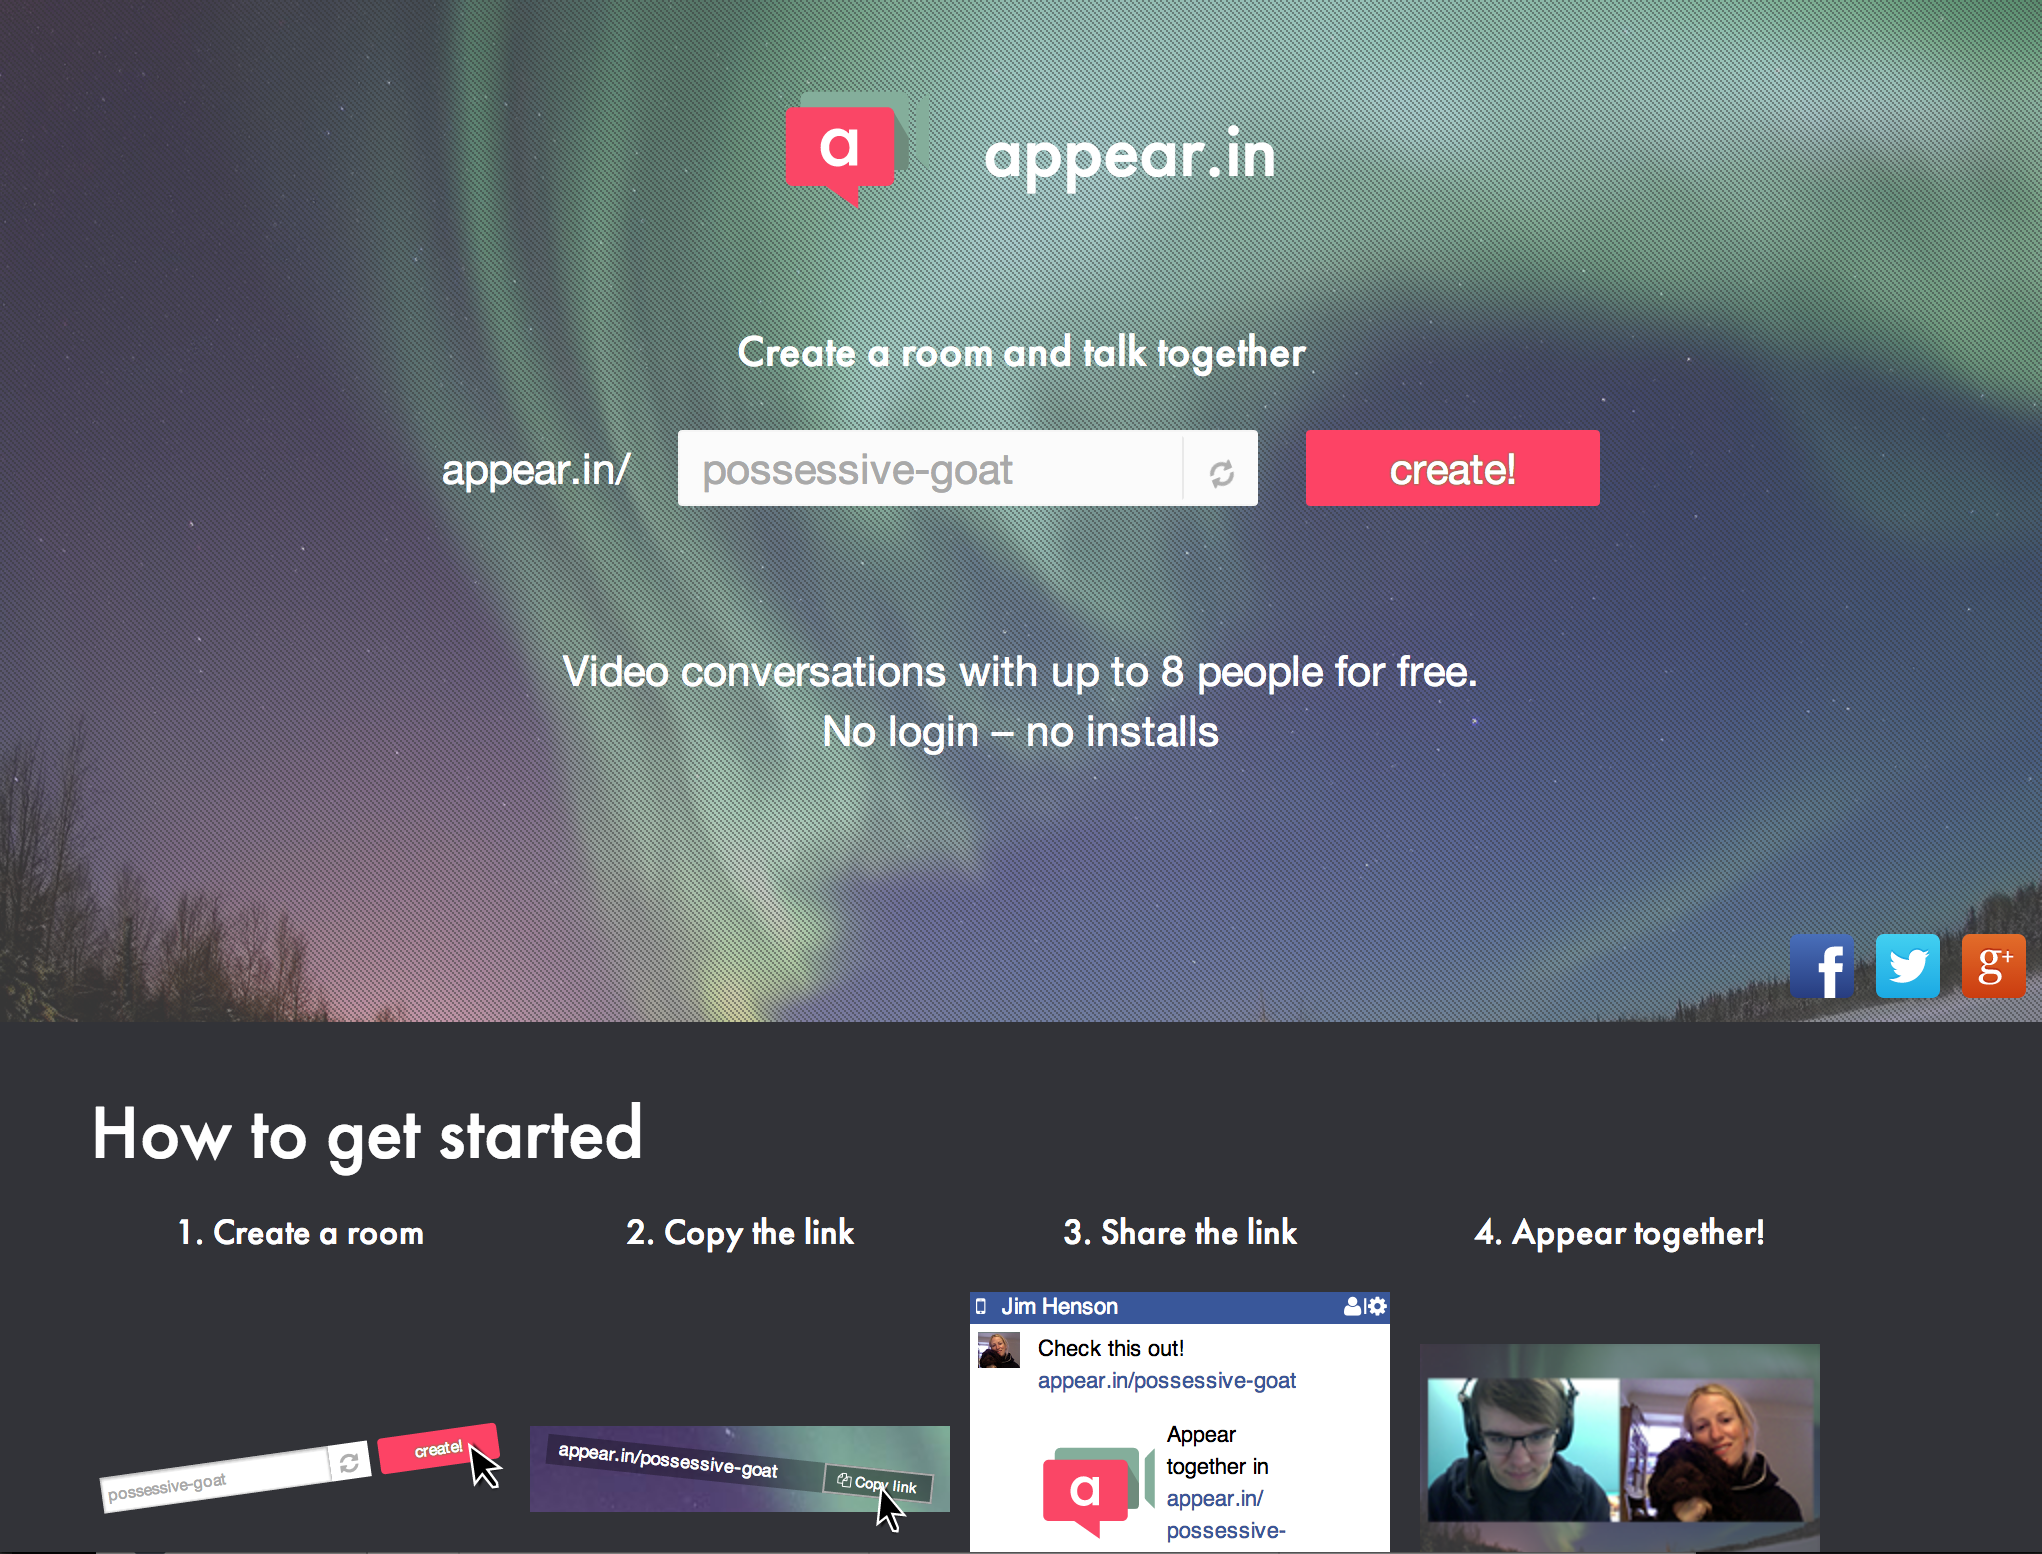
\includegraphics[width=\textwidth]{Figures/screenshots/ab-frontpage/variation-off}
      \caption{Variation $A$.}
      \label{fig:variation_a}
    \end{subfigure}

    \vspace{1em}

    \begin{subfigure}[t]{0.8\textwidth}
      \centering
      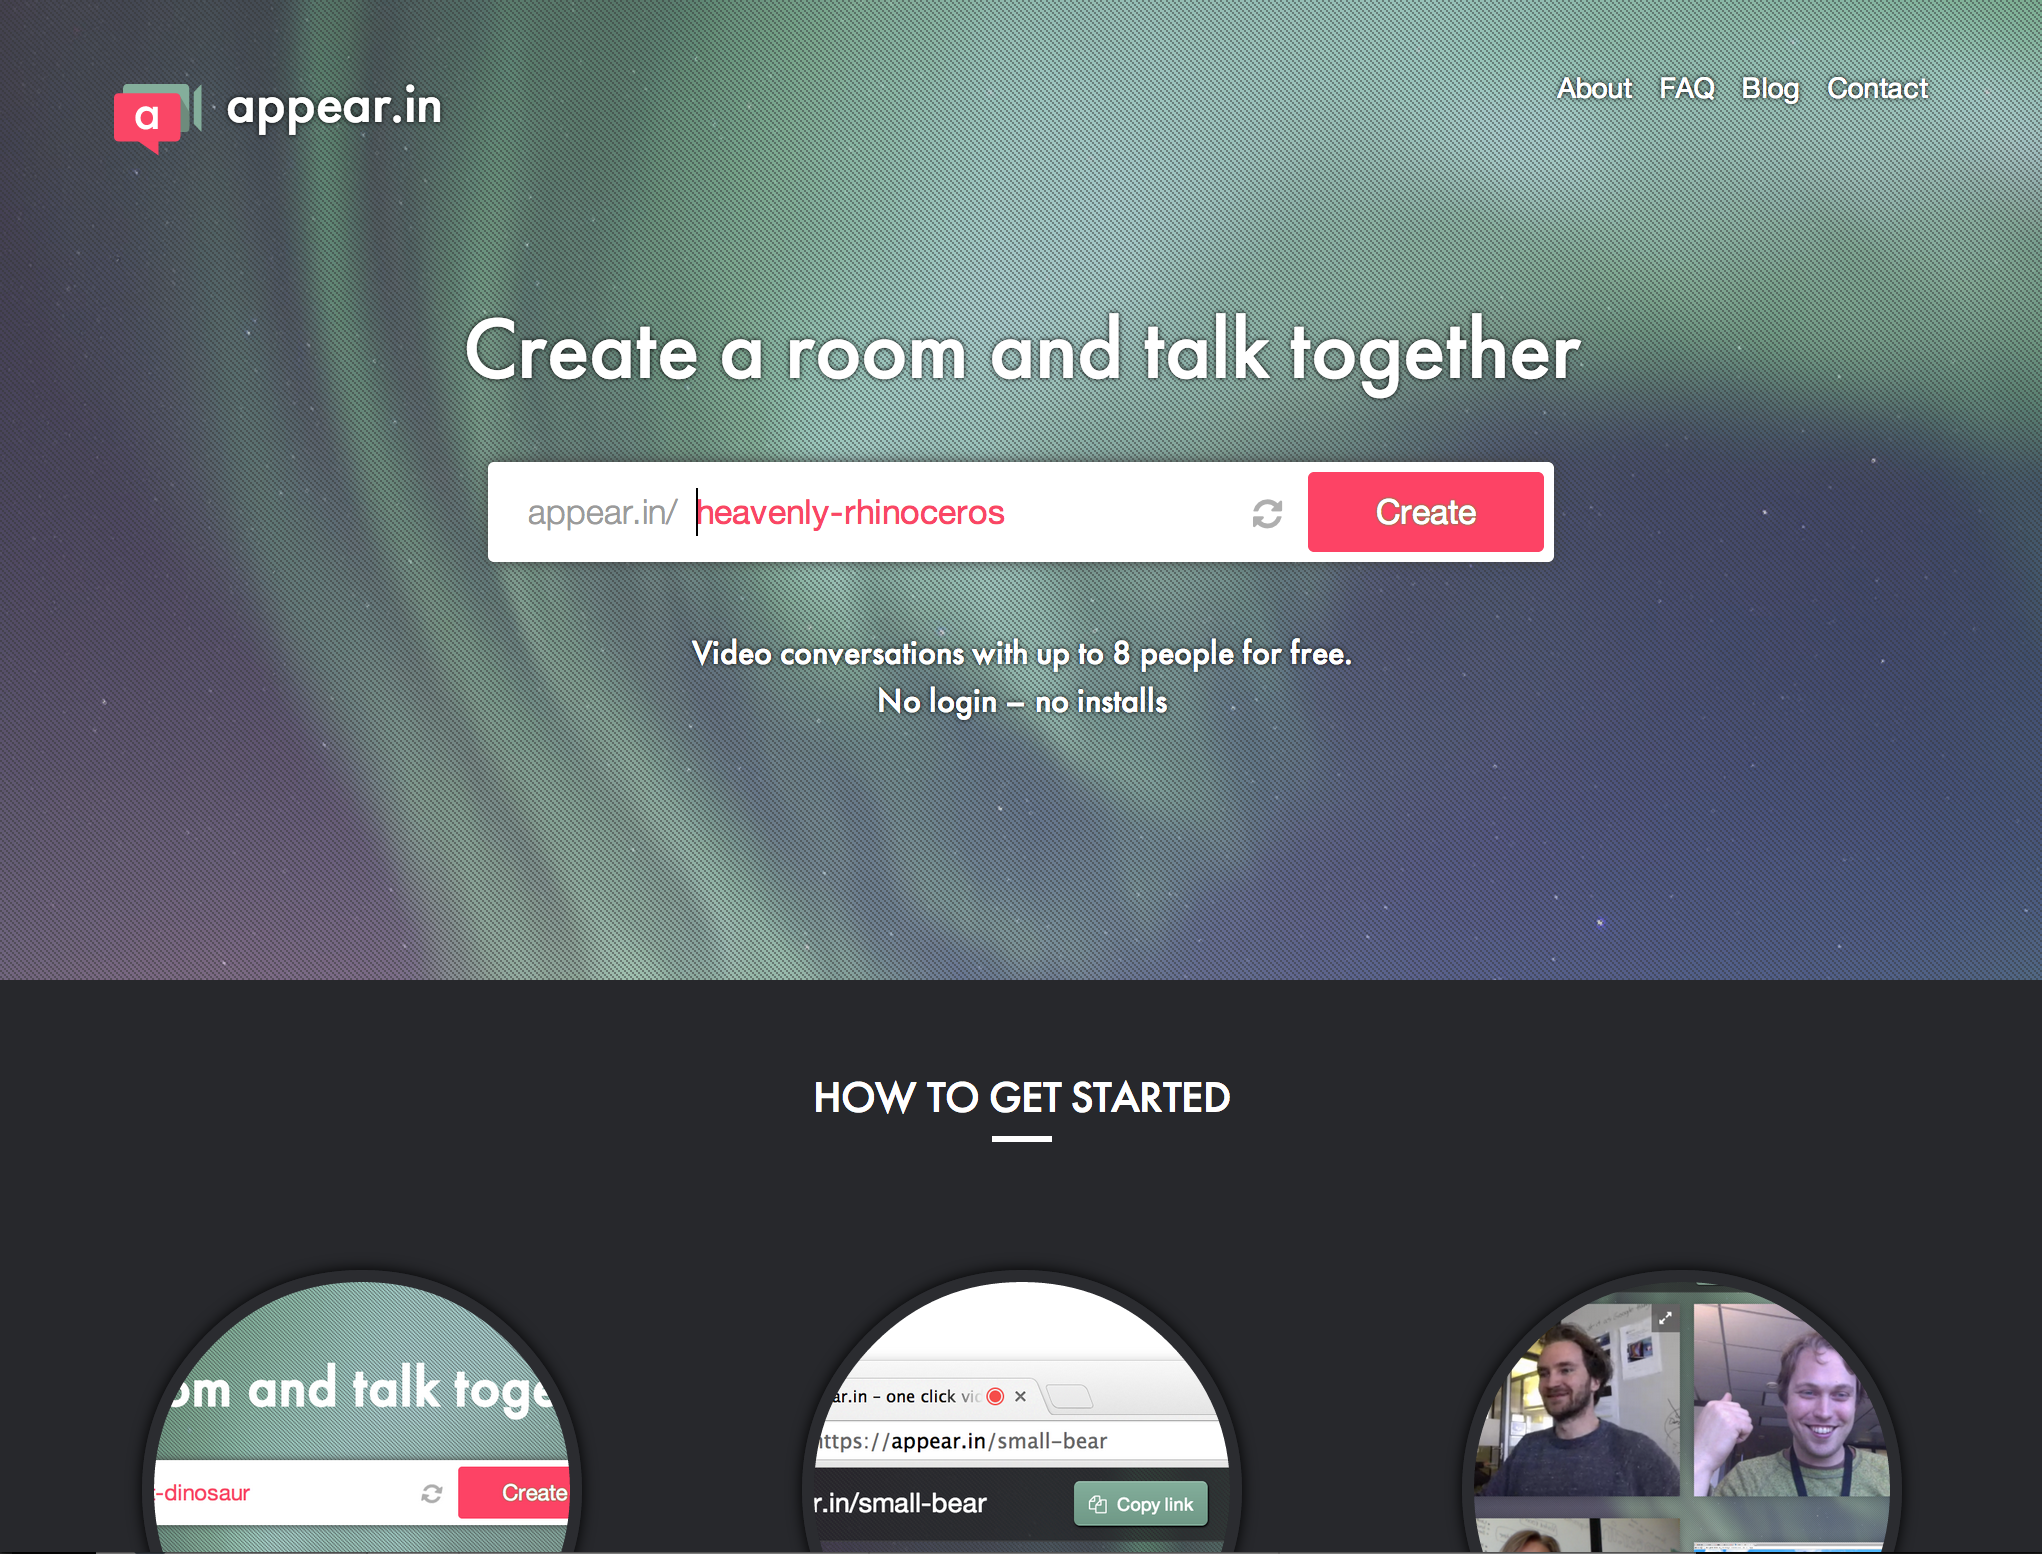
\includegraphics[width=\textwidth]{Figures/screenshots/ab-frontpage/variation-on}
      \caption{Variation $B$.}
      \label{fig:variation_b}
    \end{subfigure}

  \caption{Variations in the new landing page experiment.}
  \label{fig:variations}
\end{figure}

After running for one week with an even randomized user split between the two variations, the results were in. In total, just over 20,000 people were included in the experiment and were served one of the two variations.

The two were compared head to head for two different performance metrics:

\begin{description}
  \item[Visited room] \hfill \\
    The number of users going from the landing page and into a room.
  \item[In a conversation] \hfill \\
    The number of users going from the landing page and into a conversation. This entails that the person in question has understood the concept of how one establishes a conversation, which can be seen as the next step of user activation after entering a room.
\end{description}

Figures~\ref{fig:performance_room} and~\ref{fig:performance_conversation} show how the variations performed with respect to the two metrics, both with variation $B$ plotted relative to variation $A$ as the baseline.
The aggregate numbers are shown in tables~\ref{tab:performance_room} and~\ref{tab:performance_conversation}.

\begin{table}[h]
  \begin{tabular}{|l|r|r|r|r|r|}
    \hline
    Variation & People & Conversions & Average conversion & Improvement & Certainty \\ \hline
    $A$       & 10,100 & 7,946       & 78.67\%            & -           & -         \\ \hline
    $B$       &  9,931 & 7,883       & 79.38\%            & 0.90\%      & 89.04\%   \\ \hline
  \end{tabular}
  \caption{Comparison of ``Visited room'' conversion ratios for variations $A$ and~$B$.}
  \label{tab:performance_room}
\end{table}

\begin{table}[h]
  \begin{tabular}{|l|r|r|r|r|r|}
    \hline
    Variation & People & Conversions & Average conversion & Improvement & Certainty \\ \hline
    $A$       & 10,009 & 3,602       & 35.99\%            & -           & -         \\ \hline
    $B$       & 10,172 & 3,781       & 37.17\%            & -3.29\%     & 95.98\%   \\ \hline
  \end{tabular}
  \caption{Comparison of ``In a conversation'' conversion ratios for variations $A$ and~$B$.}
  \label{tab:performance_conversation}
\end{table}

\begin{figure}[h]
  \centering
  \begin{subfigure}[t]{0.8\textwidth}
    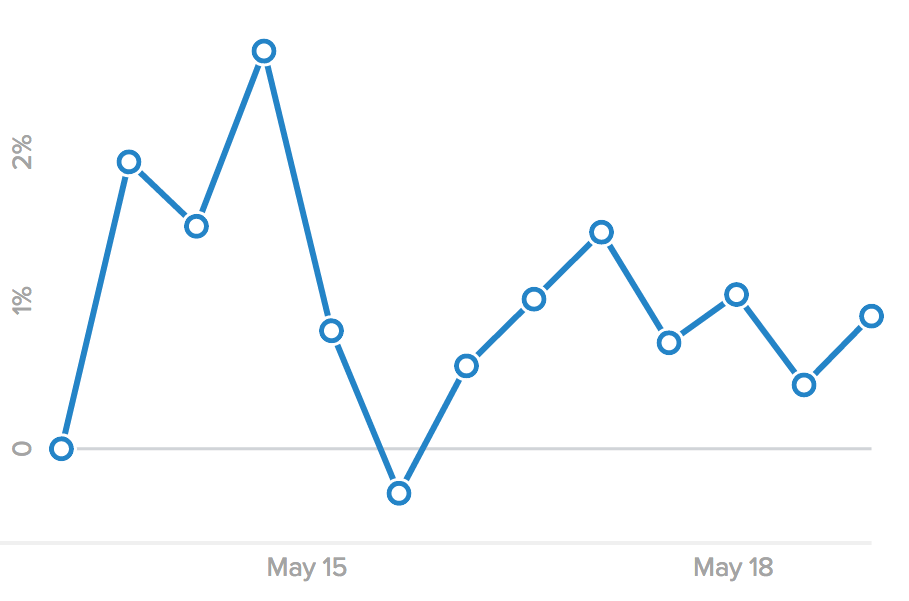
\includegraphics[width=\textwidth]{Figures/plots/ab-frontpage/room-conversions-plot-only}
    \caption{Comparison of the variations by the ``Visited room'' metric.}
    \label{fig:performance_room}
  \end{subfigure}

  \vspace{1em}

  \begin{subfigure}[t]{0.8\textwidth}
    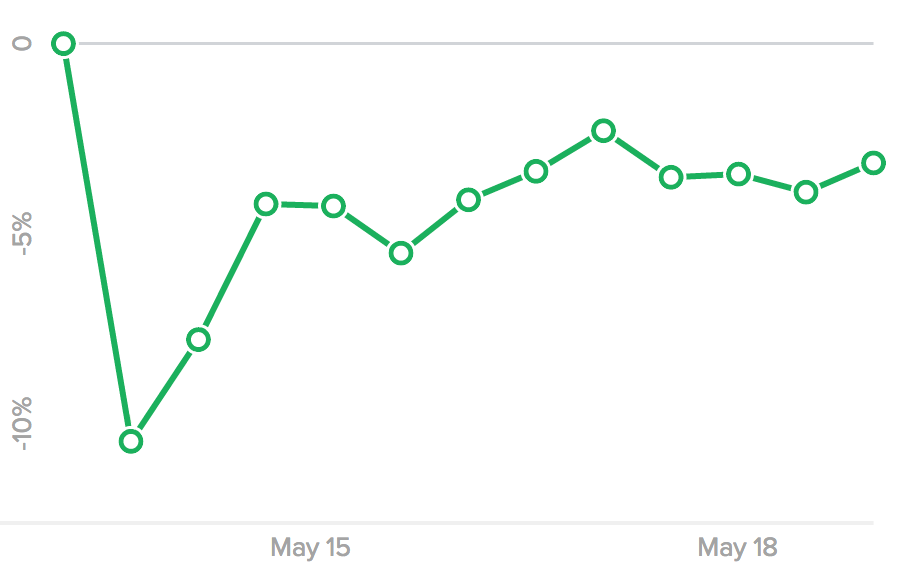
\includegraphics[width=\textwidth]{Figures/plots/ab-frontpage/conversation-conversions-plot-only}
    \caption{Comparison of the variations by the ``In a conversation'' metric.}
    \label{fig:performance_conversation}
  \end{subfigure}

  \caption{Variation $B$ performance, relative to variation $A$ (the baseline).}
  \label{fig:ab_performance_plots}
\end{figure}

As we can plainly see, variation $B$ performs slightly better at moving people into rooms, but evidently fails to communicate the conversation concept, leading to a relative decrease in actual subsequent conversations.

While these numbers and plots set the scene, they are not very interesting from our adaptation perspective. We are first and foremost interested in seeing whether these numbers vary significantly between segments of the user base, providing us with a predictive bias from which we can extrapolate our user adaptations. Section~\ref{eval:sec:adapting_the_application} breaks the numbers down cluster by cluster, and investigates to what degree this information can be used to adapt the interface.

\section{User clustering} % (fold)
\label{eval:sec:clustering}

\begin{figure}[h]
  \centering
    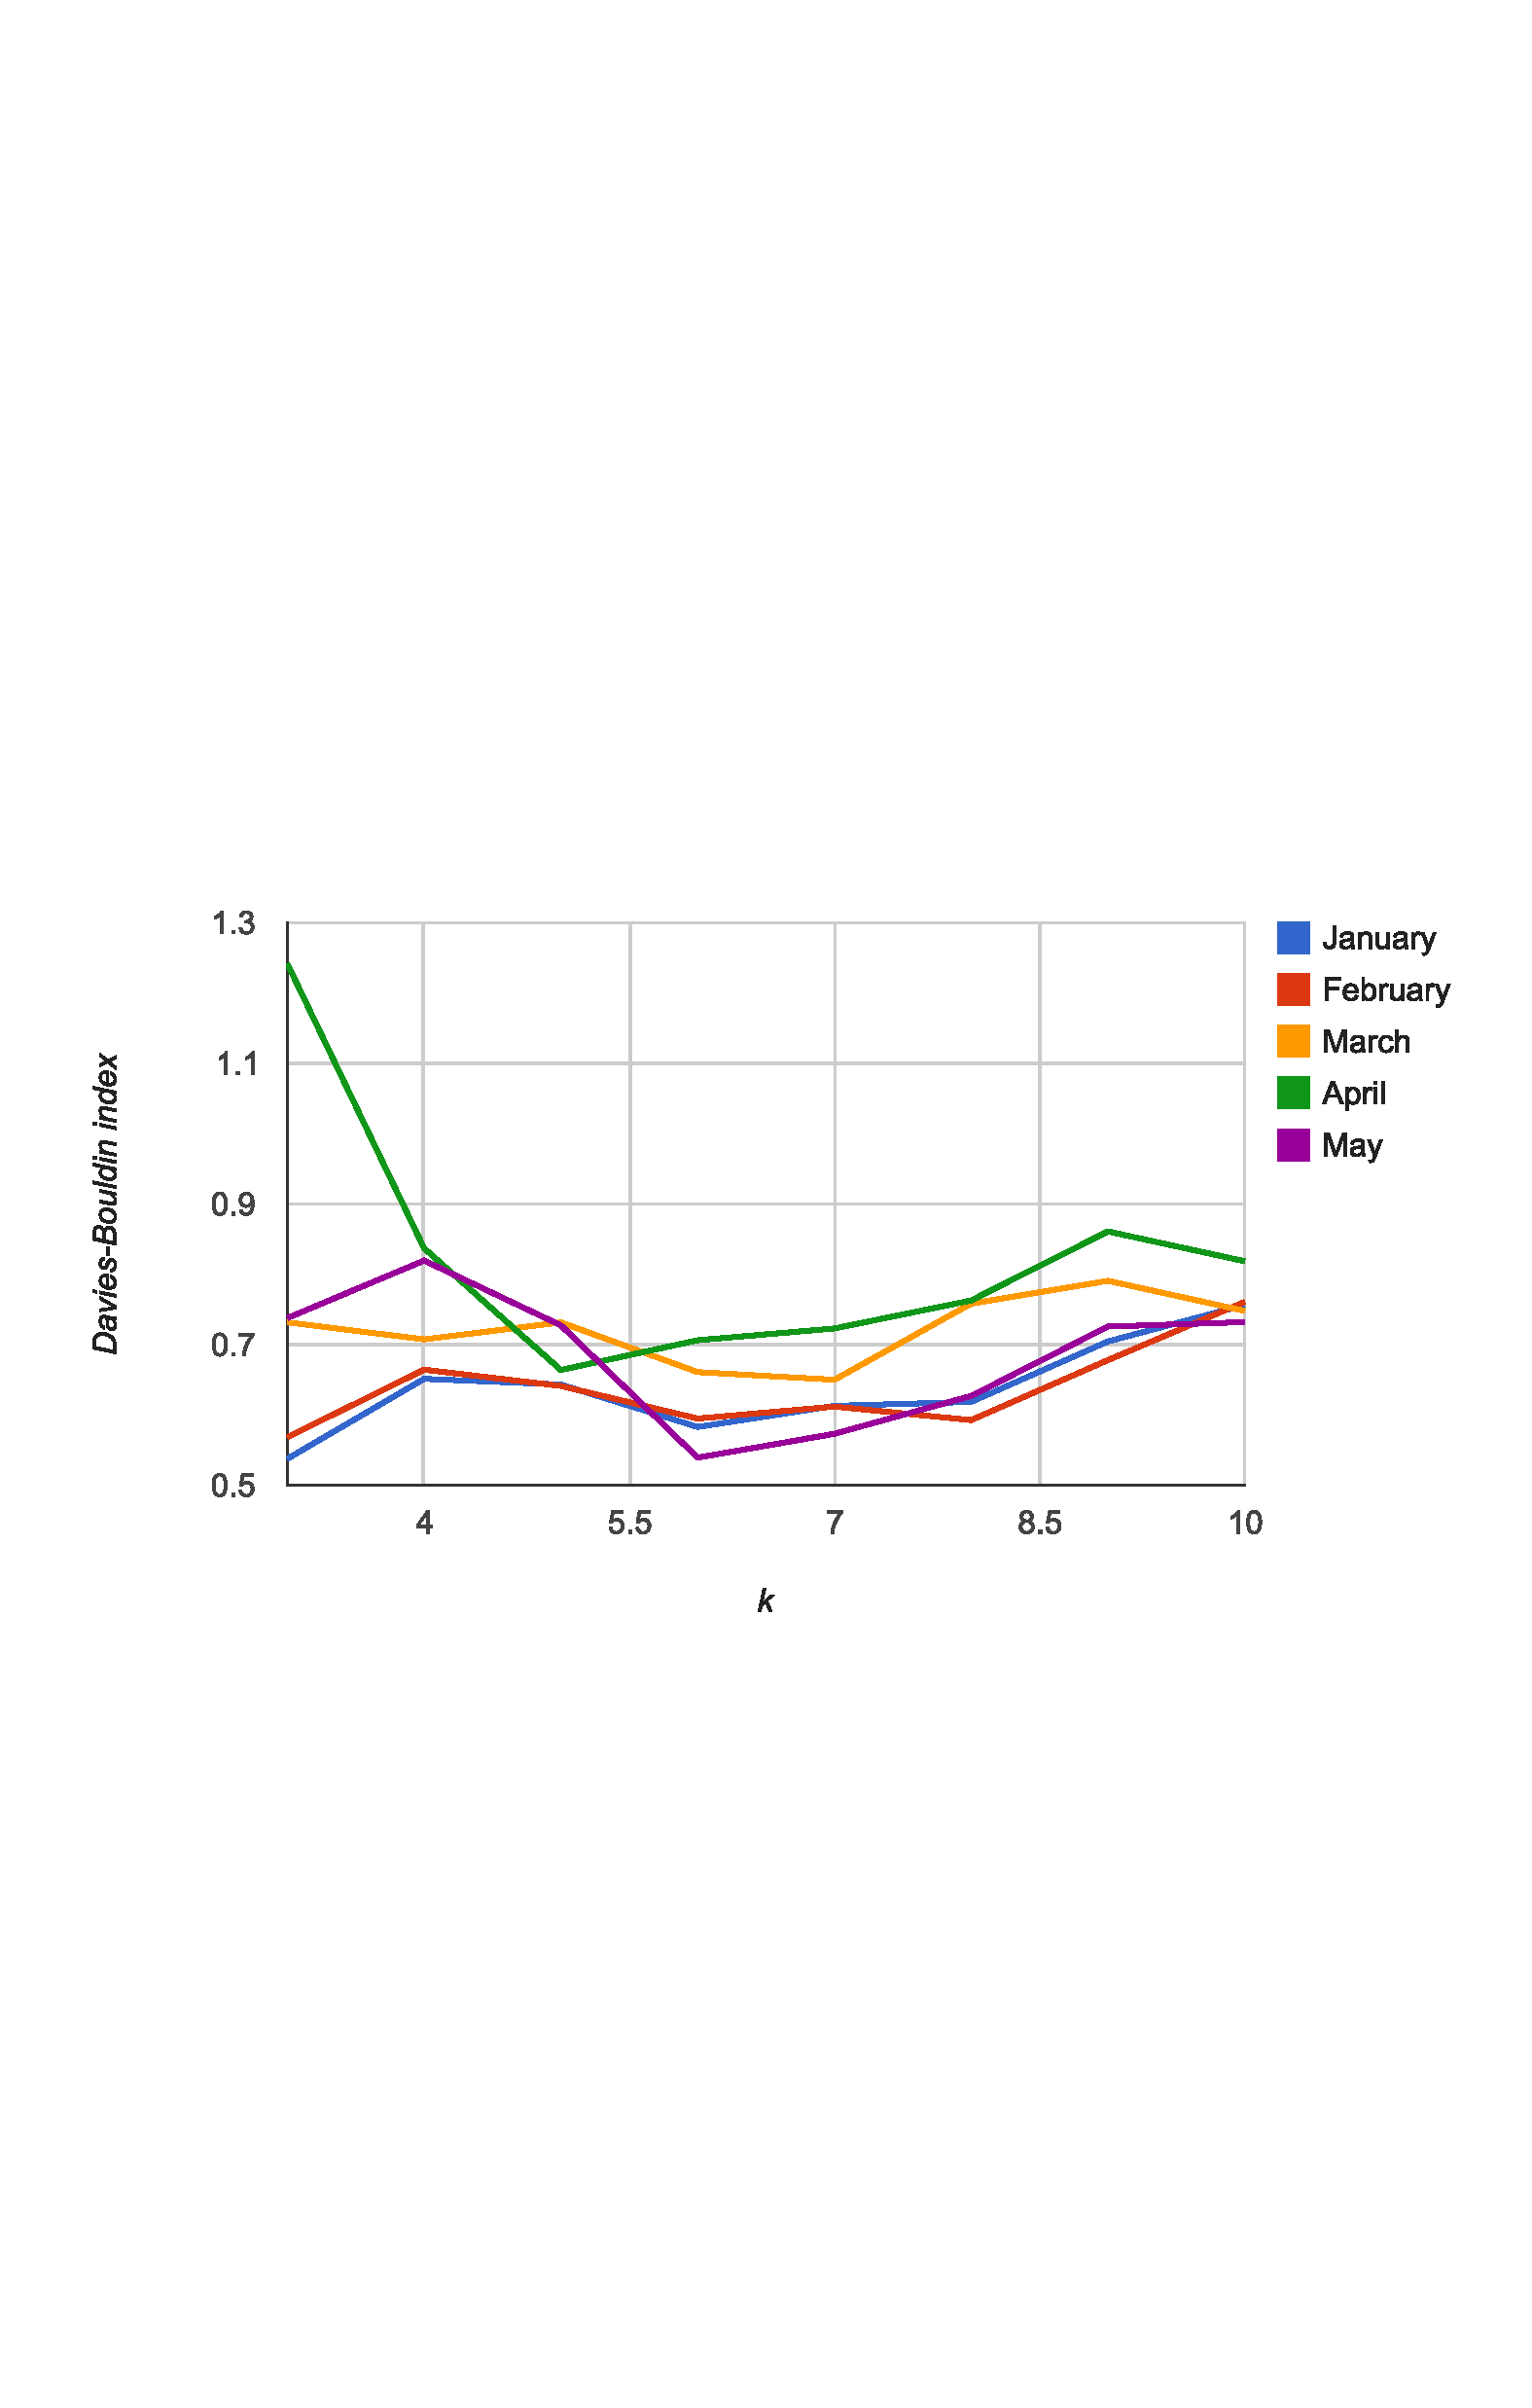
\includegraphics[width=\textwidth]{Figures/plots/k-vs-db/jan-may}
    \caption{$k$ vs. Davies-Bouldin index, for clusters with data for January to May.}
    \label{fig:k_vs_db}
\end{figure}

\emph{@TODO: Describe parameters used. What kind of results are expected?}

The clustering approach was iteratively improved on over several months. Large amounts of new data was gathered through the developments process, and with it the parameters were tuned and adapted.

The tool wrapping the k-means clustering algorithm ended up supporting the set of runtime options shown in table~\ref{tab:clustering_runtime_options}.

\begin{table}[h]
  \begin{tabular}{ll}
    \texttt{--timespan}          & Includes data only within the supplied timespan. \\
    \texttt{-k}                 & Number of clusters. \\
    \texttt{--normalize}         & Normalize axes before clustering. \\
    \texttt{--drop-zero-vectors} & Don't include user model vectors of length zero in clustering. \\
  \end{tabular}
  \caption{Runtime options for clustering algorithm.}
  \label{tab:clustering_runtime_options}
\end{table}

As different time periods saw user influx from a large variety of demographic origins (discussed in~\ref{eval:sub:varying_demographics}), the \emph{timespan} parameter was used extensively to compare these to aid in avoiding local maxima.

\subsection{Varying demographics}
\label{eval:sub:varying_demographics}

Through the spring of 2014, appear.in received quite a bit of media attention. The coverage varied from technical showcases and industry newsletters to the service being featured in Hungarian newspapers and on BBC World News.

\subsection{Initial clustering results}
\label{eval:sec:clustering_results}

The data used in this analysis stems from February 2014.

The following clustering results were found by choosing the best of 5 k-means runs, ``best'' being defined by their Davies-Bouldin indices (see section~\ref{survey:sub:clustering_evaluation} for a brief description of this evaluation metric). This process was performed for $k$ parameter values from 3 to 10, where $k = 8$ yielded the best result. The 2 smallest resulting clusters were omitted in the analysis due to their relatively insignificant sizes.

Data from January and March yield more or less the same results, although they are a bit less clear. This could be due to media events and holidays generating more skewed data than usual.

\begin{figure}[h]
  \centering
    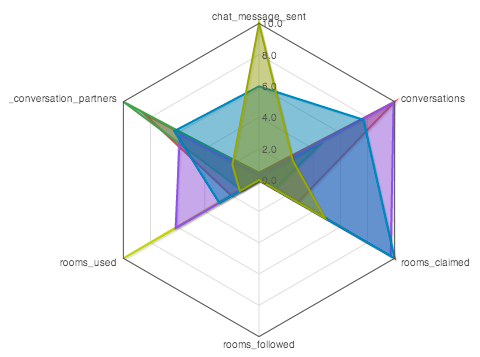
\includegraphics[width=0.8\textwidth]{Figures/clusterings/confluence-post/comp-02-feb}
    \caption{Radar chart comparing clusters generated from data for February 2014.}
    \label{fig:radar-clusters-february}
\end{figure}

The radar chart in figure~\ref{fig:radar-clusters-february} shows the centroids of 6 large clusters $C$ relative to each other.

Each dimension's centroid values $\mu_i \in \mu$ have been scaled by a factor of $\frac{10}{\max_{c \in C}{c_i}}$, to fit nicely inside the chart.

The features used in this particular clustering run are (going clockwise around the chart):

\begin{enumerate}
  \item chat messages sent
  \item conversations (2+ persons present in room)
  \item rooms claimed
  \item rooms followed
  \item unique rooms used
  \item conversation network size (ie. number of unique other users within 2 degrees of conversation separation)
\end{enumerate}

Most of these features are quantified by counting the number of relevant events logged for each user.

A ... \ref{eval:sec:clustering_results}.

\subsection{The applicability of manual cluster analysis}
\label{eval:sub:cluster_analysis_applicability}

When analyzing a set of clusters, it is tempting to focus on the extremes -- the easily stereotyped user profiles -- as we have done above. However, we see that a vast majority of users are indeed too close to the origo to be confidently labelled as some kind of stereotype.

Thus, although tempting from a business intelligence type of perspective, manual cluster stereotyping becomes a highly speculative exercise whose conclusions are extremely hard to confirm without demographic data readily available.

We will return to this issue in chapter~\ref{Chapter5}.

\section{Adapting the application} % (fold)
\label{eval:sec:adapting_the_application}

The task of adapting the application brings together previous A/B test results and the clusters discovered, as described in sections~\ref{eval:sec:ab_testing_features} and~\ref{eval:sec:clustering}.

\begin{table}
  \begin{tabular}{| lr |  rrr| rrr| rrr| c|}
\hline
 \multicolumn{2}{|l|}{Variations} & \multicolumn{3}{|c|}{off} & \multicolumn{3}{|c|}{on} & \multicolumn{3}{|c|}{total} & \\
\hline
 $C$ & $|C|$ & n & c & \% & n & c & \% & n & c & \% & preferred \\
\hline
1 & 92,762 & 42 & 0 & 0.00 & 43 & 0 & 0.00 & 85 & 0 & 0.00 & off \\
2 &  3,566 & 21 & 9 & 42.86 & 16 & 11 & 68.75 & 37 & 20 & 54.05 & on \\
3 &    607 & 156 & 75 & 48.08 & 152 & 67 & 44.08 & 308 & 142 & 46.10 & off \\
4 &    442 & 151 & 90 & 59.60 & 160 & 113 & 70.62 & 311 & 203 & 65.27 & on \\
5 &    377 & 118 & 106 & 89.83 & 133 & 125 & 93.98 & 251 & 231 & 92.03 & on \\
6 &    584 & 180 & 145 & 80.56 & 165 & 134 & 81.21 & 345 & 279 & 80.87 & on \\
\hline
\end{tabular}

% sizes: [92762, 3566, 607, 442, 377, 584]
% ids: [2135, 2136, 2137, 2138, 2139, 2140]

  \caption{A result.}
  \label{tab:results}
\end{table}

\section{Identity persistence}
\label{eval:sec:identity_persistence}

As has been discussed extensively already, a major difficulty in adapting applications such as appear.in to its users is that there is no concrete notion of \emph{a user}. Users are anonymous, and the only way they are being tracked at all is through a random hash set in a tracking cookie (see section~\ref{survey:unreliable_identity} and~\ref{survey:sec:privacy_vs_personalization}).

How, though, does this affect our adaptation efforts? One way of gauging this is to look at how many users return over time; that is, to what extent are unique cookie hashes seen over time?

Table~\ref{tab:returning_users} shows the number of unique users that visited the site in January, February and March, along with the percentage of these users who were seen again during the next 1 thru 5 months.

\begin{table}[h]
  \begin{tabular}{|l|r|rrrrr|}
    \hline
    From month & Base    & 1 month & 2 months & 3 months & 4 months & 5 months \\ \hline
    January    & 25,452  & 23.20\% & 5.10\%   & 2.90\%   & 1.90\%   & 0.90\%   \\
    February   & 26,273  & 20.20\% & 3.80\%   & 2.10\%   & 1.10\%   & -        \\
    March      & 113,715 & 23.20\% & 5.40\%   & 2.90\%   & -        & -        \\ \hline
  \end{tabular}
  \caption{Portions of identified users returning to the site over time.}
  \label{tab:returning_users}
\end{table}

Two plots of these numbers can be seen in figure~\ref{fig:perceived_user_persistence}, with normal scale and logarithmic scale.

As we see, just over 20\% are seen again the month after they first visit the site. Only about 20\% of these users again make it through to the subsequent month. After three months, less than 3\% remain in all three cases.

There are three reasons for the perceived number of users to drop:

\begin{enumerate}
  \item The user did not use the service again.
  \item The user cleared the browser cookies.
  \item The user changed browser or computer.
\end{enumerate}

There is all reason to believe that we are looking at a combination between all three factors, yet hard to know how much each contributes to the trend.

Based on the survey performed by Teltzrow and Kobsa~\cite{Teltzrow2004}, as discussed in section~\ref{survey:sec:privacy_vs_personalization}, we will assume that the last two factors contribute significantly to these numbers.

\begin{figure}[t]
  \centering
  \begin{subfigure}[t]{\textwidth}
    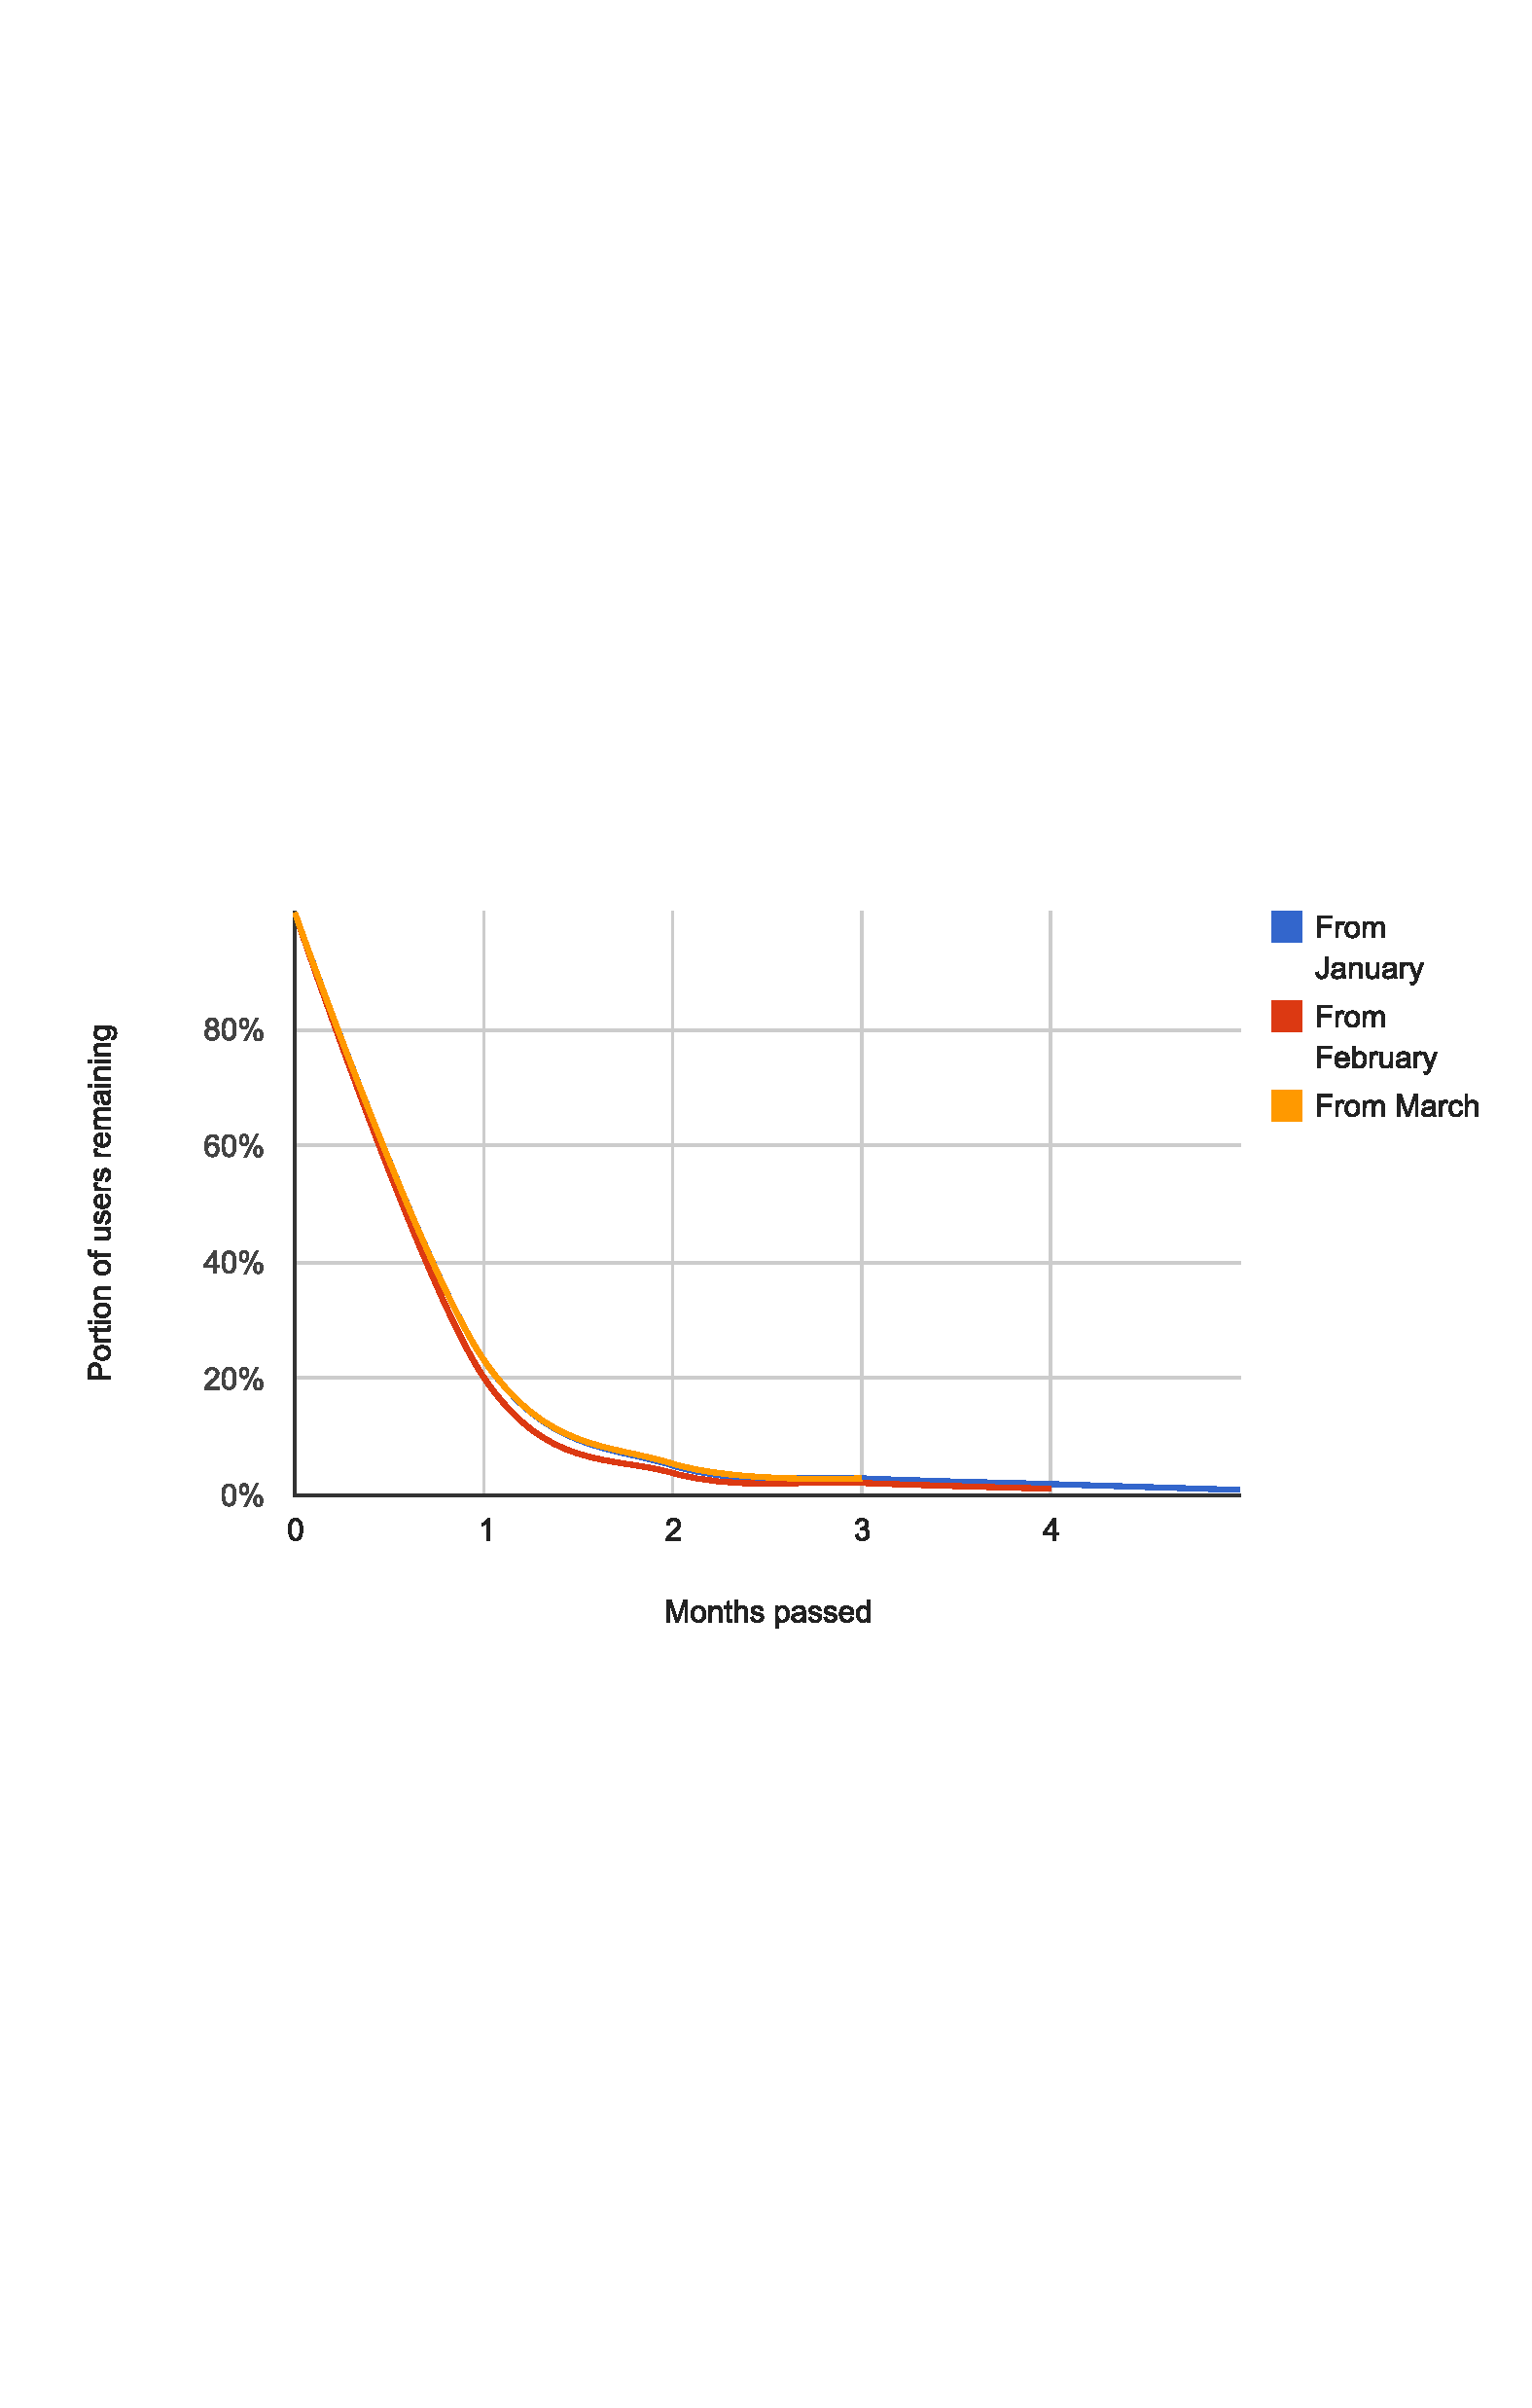
\includegraphics[width=\textwidth]{Figures/plots/user-dropoff/months-jan-mar}
    \caption{Perceived user persistence.}
  \end{subfigure}

  \vspace{1em}

  \begin{subfigure}[t]{\textwidth}
    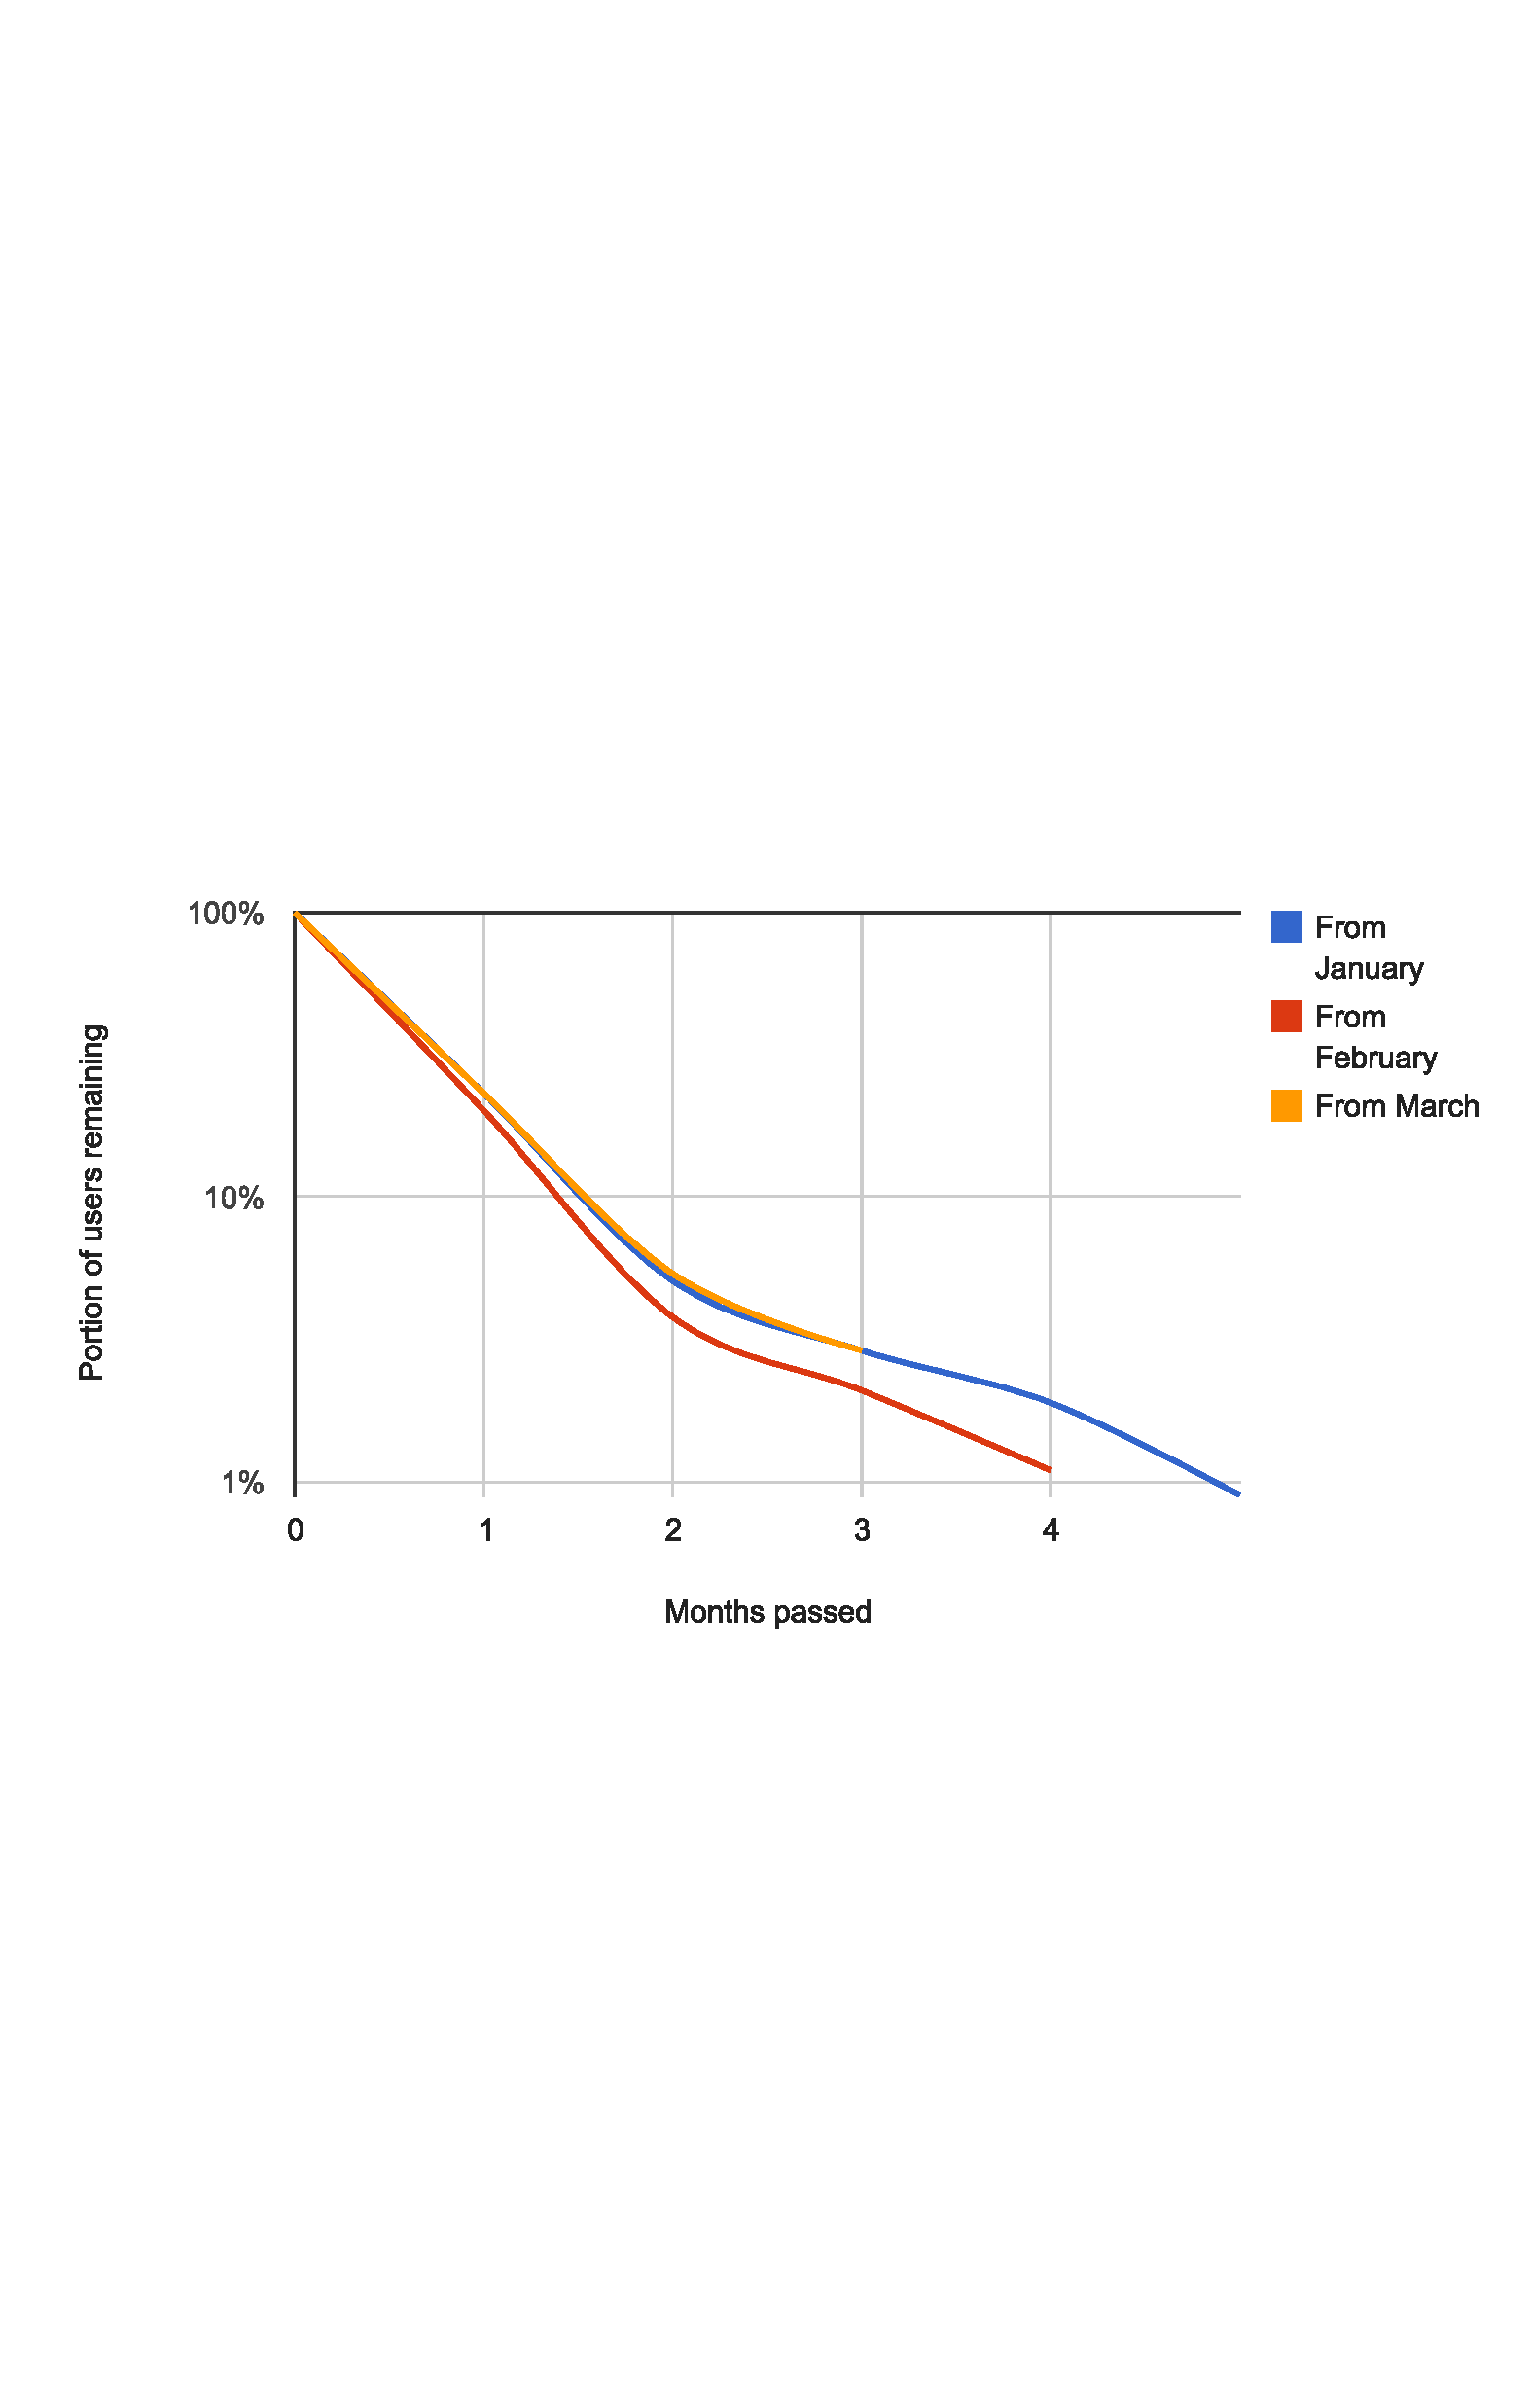
\includegraphics[width=\textwidth]{Figures/plots/user-dropoff/months-jan-mar-log}
    \caption{Perceived user persistence, logarithmic scale.}
  \end{subfigure}

  \caption{Perceived user persistence, illustrating the identified user dropoff rate.}
  \label{fig:perceived_user_persistence}
\end{figure}

\section{Summary} % (fold)
\label{eval:sec:summary}


% section results (end)

\section{Discussion} % (fold)
\label{eval:sec:discussion}

% section discussion (end)

\chapter{Evaluation}

\label{Chapter5}

\lhead{Chapter 5. \emph{Evaluation}}

% \emph{Beskriv hvordan du vurderer arbeidet ditt. Oppsummer evalueringsresultatene, og bruk dem til å vurdere ditt eget arbeid kritisk. Vær ærlig om eventuelle mangler. Hva betyr resultatene?}

\section{Evaluation metrics} % (fold)
\label{sec:evaluation_metrics}

\subsection{How to measure a positive user experience} % (fold)

% section evaluation_metrics (end)

\section{Tracking user treatments} % (fold)
\label{sec:tracking_user_treatments}

% section tracking_user_treatments (end)

\section{Visualizing effects} % (fold)
\label{sec:visualizing_effects}

% section visualizing_effects (end)



%----------------------------------------------------------------------------------------
%	THESIS CONTENT - APPENDICES
%----------------------------------------------------------------------------------------

\addtocontents{toc}{\vspace{2em}} % Add a gap in the Contents, for aesthetics

\appendix % Cue to tell LaTeX that the following 'chapters' are Appendices

% Include the appendices of the thesis as separate files from the Appendices folder
% Uncomment the lines as you write the Appendices

\chapter{Evaluation Results}

\label{AppendixA}

\lhead{Appendix A. \emph{Evaluation Results}}



% \chapter{Design Documents}

\label{AppendixB}

\lhead{Appendix B. \emph{Design Documents}}


% \chapter{Evaluation Results}

\label{AppendixC}

\lhead{Appendix C. \emph{Evaluation Results}}



\addtocontents{toc}{\vspace{2em}} % Add a gap in the Contents, for aesthetics

\backmatter

%----------------------------------------------------------------------------------------
%	BIBLIOGRAPHY
%----------------------------------------------------------------------------------------

\label{Bibliography}

\lhead{\emph{Bibliography}} % Change the page header to say "Bibliography"

\bibliographystyle{unsrtnat} % Use the "unsrtnat" BibTeX style for formatting the Bibliography

\bibliography{CustomBibliography,Bibliography}

\end{document}
